\PassOptionsToPackage{svgnames}{xcolor}
\documentclass[a4paper]{article}

\usepackage{pdp}

%------------------------------------------------------------------------------
%	REPORT INFORMATION
%------------------------------------------------------------------------------

\title{Quoridor -- Java}
\subtitle{Rapport final}
\author{Abdeldjabar Ismail Abdraman, Cengiz Vasseur, Joris Douillet, Khadidja Ahmat Hassan, Matthieu Pourageaud}

%------------------------------------------------------------------------------

\begin{document}

%------------------------------------------------------------------------------
%	TITLE P
%------------------------------------------------------------------------------

\maketitle
\thispagestyle{empty}

%------------------------------------------------------------------------------
%	MAIN MATTER
%------------------------------------------------------------------------------

\section{Explication détaillée du sujet}
\subsection{Historique du jeu Quoridor}
Le Quoridor est un jeu de stratégie qui ne fait pas intervenir de hasard et où tous les joueurs connaissent parfaitement l’état du jeu à chaque instant. Il a été créé par Mirko Marchesi dans les années 1970. On peut le comparer à des classiques comme les échecs ou le go, où la réflexion et la stratégie priment complètement sur la chance. C’est pour cette raison qu’il est particulièrement intéressant pour l’étude de l’intelligence artificielle et de la théorie des jeux.

L’origine de Quoridor remonte à un jeu plus ancien appelé \textit{Blockade}, créé par Philip Slater. Ce jeu introduisait déjà l’idée principale : utiliser des obstacles pour ralentir l’adversaire sur un plateau quadrillé. Mirko Marchesi a repris ce concept, l’a simplifié et équilibré pour qu’aucun joueur ne puisse être totalement bloqué. Dans Quoridor, un chemin vers la ligne d’arrivée doit toujours rester ouvert pour chaque joueur, ce qui distingue ce jeu de beaucoup d’autres jeux de blocage.

Le jeu a été édité et popularisé dans les années 1990 par la société Gigamic, spécialisée dans les jeux abstraits modernes. Cette période a vu l’apparition de nombreux jeux simples à comprendre mais très riches stratégiquement, et Quoridor s’inscrit parfaitement dans cette tendance avec son système minimaliste mais aux possibilités infinies.

En 1997, Quoridor a remporté le prix \textit{Mind Game}, décerné par Mensa aux États-Unis, qui récompense les jeux demandant réflexion, logique et stratégie. Cette distinction a beaucoup contribué à sa notoriété internationale. Le jeu a ensuite été élu jeu de l’année dans plusieurs pays comme la France, les États-Unis, le Canada et la Belgique, confirmant son succès auprès des joueurs occasionnels comme des amateurs de stratégie.

Le principe du jeu est simple mais efficace : chaque joueur a un pion et doit atteindre la ligne opposée du plateau tout en posant éventuellement des murs pour ralentir ses adversaires. Cette dualité entre avancer soi-même et gêner les autres oblige à adopter des stratégies à la fois offensives et défensives. Contrairement à d’autres jeux abstraits où l’objectif est de capturer des pièces adverses, Quoridor repose uniquement sur la gestion de l’espace et du temps.

Le jeu est également intéressant d’un point de vue scientifique et informatique. Le plateau peut être modélisé comme un graphe : les cases sont des nœuds et les déplacements possibles des arêtes. Les murs viennent modifier ce graphe en supprimant certaines connexions, ce qui complique l’analyse du jeu. Cette représentation permet d’utiliser des algorithmes de parcours de graphe, comme le Breadth-First Search (BFS), pour calculer les chemins les plus courts vers l’objectif.

Quoridor est souvent utilisé pour tester différentes approches d’intelligence artificielle. Sa complexité combinatoire, moins élevée que celle des échecs ou du go, reste suffisante pour rendre inefficaces les méthodes de recherche exhaustive. Cela en fait un terrain idéal pour des algorithmes comme Minimax, l’élagage alpha-bêta ou le Monte Carlo Tree Search (MCTS). La règle obligeant à laisser un chemin libre ajoute une difficulté supplémentaire pour générer et valider les coups.

Plusieurs ouvrages analysent le jeu et ses stratégies. Glendenning\cite{Glendenning2002MasteringQ} détaille les stratégies de base et insiste sur l’importance de bien choisir quand poser un mur et anticiper les actions de l’adversaire. Jose et al.\cite{jose2022quoridorai} se sont intéressés plus récemment à l’intelligence artificielle, en étudiant comment des algorithmes peuvent analyser et améliorer le jeu.

Avec l’avènement du numérique, Quoridor existe aussi sous forme d’applications mobiles, de plateformes en ligne et de projets académiques. Ces versions ont permis d’élargir le nombre de joueurs et de tester de nouvelles approches algorithmiques. Elles permettent aussi de collecter des données de jeu pour faire des analyses statistiques ou de l’apprentissage automatique.

Le jeu est aussi utilisé dans l’enseignement pour illustrer des concepts en informatique : graphes, algorithmes de recherche, complexité algorithmique ou systèmes multi-agents. Comme le souligne Heliotis et al.\cite{bezakova2014}, les jeux de plateau sont un excellent support pour apprendre la stratégie algorithmique et la logique.

Enfin, Quoridor est un excellent choix pour un projet informatique, car il combine plusieurs aspects : modélisation d’un système complexe, implémentation d’algorithmes de recherche, gestion de l’interface utilisateur et conception logicielle. Il est simple à comprendre mais offre une grande profondeur stratégique et un intérêt scientifique certain. Son histoire, sa popularité et les recherches qui lui sont consacrées montrent qu’il reste un jeu adapté aux défis contemporains, notamment en intelligence artificielle.

\subsection{Principe général du jeu}

Quoridor se joue sur un plateau carré composé de 9 × 9 cases dans sa version classique. Dans le cadre de notre projet, nous avons également envisagé des variantes avec des tailles différentes, allant de 3 × 3 à 15 × 15, à condition que la taille reste impaire. Cela permet de garder un bon équilibre entre les joueurs, car chacun part avec les mêmes chances.

Le jeu peut se jouer à deux, trois ou quatre joueurs. Dans une partie à 2, 3 ou 4 joueurs, chacun commence sur une ligne opposée du plateau. Chaque joueur possède un pion qui représente sa position sur le plateau, ainsi qu’un certain nombre de murs. Au total, il y a 20 murs dans la partie, répartis entre les joueurs.

Le but du jeu est simple : être le premier à atteindre la ligne opposée à celle de départ. Même si cet objectif paraît facile à comprendre, le jeu devient rapidement complexe, car les joueurs peuvent se gêner entre eux.

À chaque tour, un joueur a deux choix possibles. Il peut soit déplacer son pion, soit poser un mur. Le déplacement se fait d’une seule case à la fois, vers le haut, le bas, la gauche ou la droite, à condition qu’il n’y ait pas de mur qui bloque le passage. Ce déplacement permet d’avancer vers l’objectif.

L’autre possibilité est de poser un mur. Les murs servent à ralentir les adversaires en bloquant certains chemins. Ils doivent être placés entre les cases, soit horizontalement soit verticalement. Il est impossible de les placer en diagonale. Une fois posé, un mur ne peut plus être déplacé ni retiré. Cela oblige les joueurs à bien réfléchir avant de les utiliser, car ils sont en nombre limité.

Une règle très importante du jeu est qu’il est interdit de bloquer complètement un joueur. Autrement dit, il doit toujours exister au moins un chemin qui lui permet d’atteindre sa ligne d’arrivée. Cette règle est essentielle, car elle garantit que la partie peut toujours continuer jusqu’à ce qu’un joueur gagne.

Le jeu repose donc sur un équilibre entre avancer et bloquer les autres. Si un joueur se concentre uniquement sur sa progression, il risque de laisser ses adversaires avancer trop facilement. À l’inverse, s’il utilise trop de murs pour bloquer les autres, il peut ralentir sa propre progression ou se retrouver sans ressources en fin de partie.

Dans les parties à plusieurs joueurs, la stratégie devient encore plus intéressante. En effet, chaque joueur doit faire attention à plusieurs adversaires en même temps. Parfois, bloquer un joueur peut en aider un autre sans le vouloir. Il faut donc bien observer la situation et adapter sa stratégie en permanence.

D’un point de vue informatique, le plateau peut être vu comme un réseau de cases reliées entre elles. Les déplacements correspondent aux chemins possibles, et les murs viennent modifier ces chemins. Cela permet d’utiliser des algorithmes pour calculer les meilleurs trajets ou vérifier que les règles sont respectées.

En résumé, Quoridor est un jeu simple à comprendre mais difficile à maîtriser. Il demande à la fois de réfléchir à ses propres déplacements et d’anticiper ceux des autres joueurs. C’est ce mélange qui rend le jeu intéressant et qui explique pourquoi il est souvent utilisé dans des projets liés à l’intelligence artificielle.
\subsection{Règles du jeu}

Le Quoridor est un jeu de stratégie dont les règles sont simples à comprendre, mais dont la profondeur stratégique est très importante. Il se joue sur un plateau carré de 9 × 9 cases (des variantes existent avec des plateaux plus petits ou plus grands tant que la taille reste impaire comme nous l'avons fait ci-dessus). Le but principal est de déplacer son pion depuis sa ligne de départ jusqu’à la ligne opposée avant les autres joueurs. Le jeu se joue à deux ou à quatre joueurs, et chaque joueur dispose d’un nombre limité de murs pour ralentir ses adversaires. Pour gagner, il faut combiner habilement déplacements et placement de murs.

\subsubsection{Déplacement des pions}

Chaque joueur possède un pion qu’il déplace à son tour. Les déplacements sont très stricts : le pion peut avancer d’une seule case à la fois, soit vers l’avant, l’arrière, à gauche ou à droite. Il n’est jamais permis de déplacer son pion en diagonale sauf dans des situations spécifiques (que nous détaillerons plus bas). De plus, un pion ne peut jamais sortir du plateau.

Le pion ne peut pas passer à travers un mur. Si un mur se trouve directement sur le chemin, le pion est obligé de s’arrêter avant celui-ci. Cela signifie qu’un mur agit comme un véritable obstacle physique qui bloque le passage, ce qui rend le placement stratégique des murs crucial pour ralentir un adversaire.

Enfin, une règle fondamentale est qu’une case ne peut jamais contenir deux pions en même temps. Cela signifie qu’il n’est pas possible de "marcher sur un autre pion" ou de l’éliminer. Chaque pion occupe sa propre case et les joueurs doivent planifier leurs déplacements en tenant compte de la position des adversaires.

\paragraph{Cas particulier : saut par-dessus un pion}
Si le pion d’un autre joueur se trouve juste devant le pion du joueur actif, il est possible de le sauter. Ce saut permet de se déplacer de deux cases d’un coup, en "franchissant" le pion qui bloque le chemin. Cela ne peut se faire que si aucune autre barrière (mur ou bord du plateau) ne bloque directement l’espace derrière le pion à sauter.

\paragraph{Saut diagonal}
Dans le cas où le pion est bloqué par un autre pion et qu’un mur ou le bord du plateau empêche de sauter directement derrière le pion, le joueur peut effectuer un déplacement en diagonale. Cette règle donne une flexibilité stratégique intéressante, car elle permet d’éviter les situations où un pion serait complètement coincé par les autres. Les déplacements diagonaux ne sont donc pas une option de base mais une solution spéciale pour résoudre des situations de blocage (Fig.~\ref{fig:regles_specifiques}).
\begin{figure}[H]
    \centering
    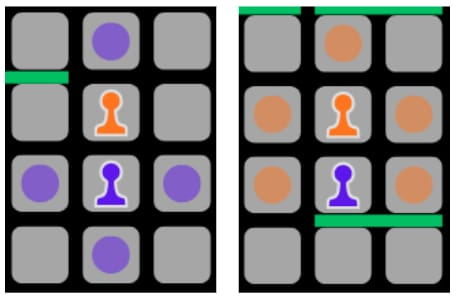
\includegraphics[width=0.6\linewidth]{regles3}
    \caption{Déplacement diagonal (saut d'un joueur)}
    \label{fig:regles_specifiques}
\end{figure}

\subsubsection{Pose des murs}

Chaque joueur dispose d’un certain nombre de murs à poser. Le placement des murs est soumis à des règles strictes qui garantissent l’équité du jeu et empêchent de bloquer complètement un adversaire.

\paragraph{Règles de base pour placer un mur}
Un mur doit toujours bloquer exactement deux cases adjacentes (voir Fig.~\ref{fig:position_normale} et Fig.~\ref{fig:murs_interdits}). Il ne peut jamais être posé en diagonale ni traverser le plateau de façon irrégulière. Un mur posé reste définitivement sur le plateau et ne peut pas être déplacé ou retiré.

Un point fondamental est que le placement d’un mur ne doit jamais empêcher un joueur d’atteindre sa ligne d’arrivée. Autrement dit, il est impossible d’enfermer un joueur entre quatre murs ou de bloquer complètement toutes les routes possibles vers la victoire. Cette règle est cruciale pour que le jeu reste équitable et stratégique.

\paragraph{Impact stratégique des murs}
Les murs permettent de ralentir un adversaire ou de forcer un joueur à modifier sa trajectoire. Bien placés, ils peuvent obliger l’adversaire à prendre un chemin beaucoup plus long et ainsi offrir un avantage stratégique. Cependant, poser un mur n’est jamais gratuit : chaque joueur dispose d’un nombre limité de murs, il faut donc les utiliser avec parcimonie et intelligence.
\begin{figure}[H]
    \centering
    \begin{minipage}{0.35\textwidth}
        \centering
        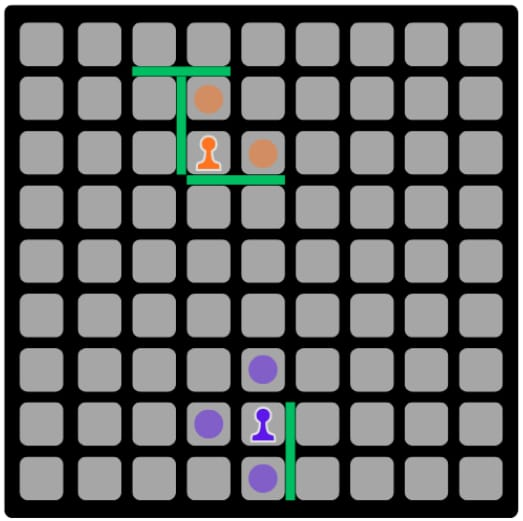
\includegraphics[width=\linewidth]{regles1}
        \caption{Position de jeu normale}
        \label{fig:position_normale}
    \end{minipage}
    \hfill
    \begin{minipage}{0.35\textwidth}
        \centering
        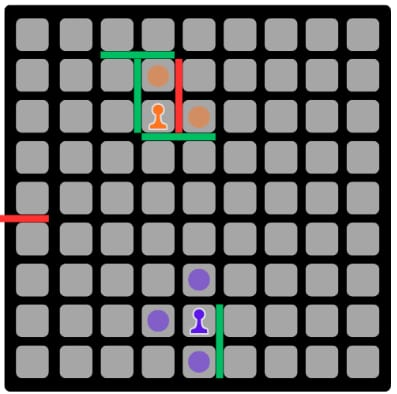
\includegraphics[width=\linewidth]{regles2}
        \caption{Murs interdits}
        \label{fig:murs_interdits}
    \end{minipage}
\end{figure}

\subsubsection{Interactions entre pions et murs}

L’une des subtilités de Quoridor réside dans la combinaison des déplacements des pions et des murs. Le joueur doit toujours prévoir plusieurs coups à l’avance pour éviter de se retrouver bloqué et pour optimiser la trajectoire de son pion tout en gênant ses adversaires.

Par exemple, si un adversaire est proche de votre ligne de départ, il peut être judicieux de poser un mur pour l’obliger à faire un détour. À l’inverse, il peut être plus avantageux de concentrer ses murs sur des zones où plusieurs pions se croisent afin de créer des effets combinés, obligeant plusieurs adversaires à changer leur chemin.

\subsubsection{Limitations et contraintes}

Le Quoridor impose plusieurs contraintes fondamentales pour maintenir l’équilibre du jeu et éviter les abus tactiques. La première contrainte majeure est la gestion des ressources : chaque mur représente une ressource rare et précieuse. Comme leur nombre est limité, chaque pose doit être mûrement réfléchie, car un mur utilisé trop tôt peut manquer d'impact, tandis qu'une économie excessive peut laisser l'adversaire prendre une avance irrattrapable. Cette pression est renforcée par la permanence des actions ; contrairement aux déplacements de pions, la pose d'un mur est définitive. Un mur ne peut être ni déplacé ni retiré, rendant toute erreur de placement irréversible et potentiellement préjudiciable pour celui qui l'a commise.

Par ailleurs, l'intégrité du chemin constitue une règle inviolable : il doit toujours exister au moins un accès libre vers la ligne d’arrivée pour chaque joueur, interdisant ainsi tout enfermement total. Enfin, des contraintes physiques simples régissent le plateau : une case ne peut être occupée que par un seul pion à la fois, et aucun élément — pion ou mur — ne peut sortir des limites strictes du jeu. Ces limitations forcent les joueurs à planifier leurs actions avec rigueur tout en respectant l'espace de liberté des adversaires.

\subsubsection{Aspects tactiques}

Ces règles simples cachent une richesse stratégique immense qui s'intensifie selon le nombre de participants. Le joueur doit constamment arbitrer entre deux objectifs contradictoires : avancer son propre pion pour se rapprocher de la victoire ou poser un mur pour entraver la progression adverse. Dans une partie à deux joueurs, la stratégie est directe et repose sur l'anticipation réciproque. En revanche, le passage à quatre joueurs transforme radicalement la dynamique du jeu. Chaque participant doit alors surveiller trois adversaires simultanément, ce qui réduit le contrôle individuel sur l'évolution du plateau. Un mur placé pour ralentir un concurrent peut involontairement ouvrir une voie royale à un autre, ou forcer un détour imprévu pour celui qui l'a posé. Cette dimension multi-joueurs impose une vigilance constante et une adaptabilité permanente aux actions often imprévisibles des autres.

La gestion du rapport bénéfice/risque est au cœur de chaque décision. Faut-il économiser ses murs pour la fin de partie ou tenter de bloquer l'adversaire dès les premiers tours ? La réponse dépend non seulement de la position des pions, mais aussi de la psychologie des adversaires et de la vision globale de l'espace de jeu. Cette combinaison de simplicité mécanique et de profondeur décisionnelle fait de Quoridor un excellent terrain pour l'étude de la planification stratégique.

\subsubsection{Conclusion sur les règles}

En résumé, Quoridor repose sur des règles simples mais exigeantes : chaque pion se déplace d'une case, les murs sont limités et doivent être placés avec prudence, et il faut toujours laisser un chemin libre pour tous les joueurs. Les règles sur le saut et le saut diagonal ajoutent des subtilités qui enrichissent la stratégie. Cette combinaison de simplicité et de profondeur stratégique fait de Quoridor un jeu accessible mais riche, parfaitement adapté à l'étude des stratégies, à l'intelligence artificielle et à la réflexion logique.

\subsection{Analyse de la complexité du jeu}

Le \emph{Quoridor} est classé parmi les jeux à haute complexité combinatoire, se situant entre les échecs et le jeu de Go en raison de la nature hybride de ses coups. Le plateau comporte 81 cases. Avec deux pions, on obtient $81 \times 80 = 6480$ positions distinctes. Il existe 64 points d'intersection pour les murs, chacun pouvant être orienté verticalement ou horizontalement, soit 128 possibilités. En prenant en compte 20 murs, et en utilisant la formule de Mertens :
\begin{equation}
S_f = \sum_{n=0}^{20} \left( \prod_{i=0}^{n-1} (128 - 4i) \right)
\end{equation}
on peut estimer la complexité de l'espace d'états à environ $10^{42}$ \cite{mertens2006}. Le facteur de branchement moyen est estimé à $\sim 60$ \cite{Glendenning2002MasteringQ}, contre 35 pour les échecs. Une partie dure en moyenne 100 demi-coups, ce qui donne une complexité totale de l'arbre de jeu de $60^{100} \approx 10^{177}$.

\subsection{Jeux ou implémentations existantes}

Le jeu Quoridor, bien qu’il soit souvent associé à une version physique vendue en boutique, existe aujourd’hui sous de très nombreuses formes, que ce soit sous forme matérielle traditionnelle, dans des versions numériques, ou encore comme point de départ pour des projets informatiques ou de recherche. Cette diversité d’implémentations montre à la fois l’accessibilité du jeu et l’intérêt qu’il suscite, non seulement parmi les amateurs de jeux de société, mais aussi au sein de la communauté scientifique et de celle des développeurs.

\paragraph{Le jeu physique traditionnel}

Dans sa forme la plus classique, Quoridor est distribué par des éditeurs de jeux de société et se trouve facilement à l’achat dans de nombreuses boutiques spécialisées ou en ligne. Ce jeu se compose d’un plateau de 9 × 9 cases, de pions pour les joueurs et d’un ensemble de murs en bois ou en plastique. La simplicité de son matériel contraste avec la profondeur stratégique qu’il offre. C’est un jeu abstrait accessible qui peut être appris en quelques minutes, mais qui peut demander des dizaines d’heures d’entraînement pour être maîtrisé. Cette accessibilité et cette profondeur expliquent en grande partie pourquoi il a su conquérir un public large, des joueurs occasionnels aux passionnés de stratégie.

L’un des signes de la reconnaissance du jeu est son prix \textit{Mind Game}, décerné en 1997 par l’association Mensa, qui récompense les jeux faisant appel à la réflexion et à la logique. Cette distinction a contribué à sa diffusion internationale, ainsi qu’à sa réputation comme un jeu stimulant et intellectuellement exigeant.

\paragraph{Versions en ligne et communautés de joueurs}

Avec le développement des technologies numériques, Quoridor a très vite été adapté en versions informatiques. Aujourd’hui, il existe de nombreuses plateformes en ligne où il est possible de jouer à Quoridor gratuitement contre d’autres joueurs à travers le monde.

Ces environnements en ligne offrent plusieurs avantages par rapport à la version physique. Premièrement, ils garantissent une \textbf{accessibilité immédiate} puisqu'il n'y a nul besoin d'acheter un plateau physique ; un simple navigateur suffit. Deuxièmement, le \textbf{matchmaking automatisé} permet de jumeler les joueurs par niveau pour affronter des adversaires de force comparable. Troisièmement, l'\textbf{analyse des parties} via l'historique ou un système de replay est extrêmement utile pour apprendre. Enfin, des \textbf{statistiques et un classement} ELO permettent de suivre sa progression au sein d'une communauté active.

Ces adaptations numériques ont grandement contribué à la popularité actuelle de Quoridor, en particulier auprès d’un public jeune et connecté. Elles ont aussi facilité l’organisation de tournois, de défis et d’événements en ligne autour du jeu, ce qui a favorisé l’émergence d’une communauté active autour de Quoridor.

\paragraph{Implémentations open‑source et projets personnels}

Au‑delà des versions commerciales et des plateformes en ligne, le jeu a inspiré de nombreux passionnés à créer leurs propres implémentations. Sur des plateformes de partage de code telles que GitHub, il est possible de trouver plusieurs projets qui reproduisent ou étendent Quoridor dans des langages de programmation variés.


Deux exemples de projets particulièrement intéressants illustrent cette diversité. \textbf{Le dépôt de \textit{alainrinder}}, disponible à l’adresse \href{https://github.com/alainrinder/quoridor.py}{\url{https://github.com/alainrinder/quoridor.py}}, propose une implémentation en Python avec interface graphique, idéale pour étudier le jeu ou développer une IA. Parallèlement, \textbf{le dépôt de \textit{pavlosdais}}, accessible sur \href{https://github.com/pavlosdais/Quoridor}{\url{https://github.com/pavlosdais/Quoridor}}, propose une version en langage C fonctionnant dans le terminal, utile pour comprendre les mécanismes internes et implémenter des moteurs légers.

Ces projets sont des ressources précieuses pour les développeurs, car ils permettent de manipuler directement les structures de données associées aux plateaux, aux pions et aux murs. Ils servent aussi de point de départ pour expérimenter différentes stratégies d’IA ou pour intégrer le jeu dans des environnements plus larges.

En complément de ces projets open‑source, on trouve également des tutoriels, des vidéos explicatives et des projets didactiques réalisés par des amateurs. Par exemple, une vidéo YouTube montre comment coder le jeu en Python en utilisant un environnement Jupyter Notebook (\href{https://youtu.be/KlktFXtj_qk?si=NpsYhWHdBjuhytDP}{voir la vidéo}). Ce type de contenu est particulièrement utile pour les débutants qui souhaitent comprendre les bases de l’implémentation du jeu sans partir de zéro.

\paragraph{Travaux scientifiques sur Quoridor et agents de jeu}

Quoridor n’est pas seulement un jeu de société apprécié des joueurs ; il a aussi attiré l’attention des chercheurs en intelligence artificielle et en informatique théorique. La raison principale est que, malgré sa simplicité apparente, Quoridor offre une complexité stratégique significative qui en fait un excellent test pour des méthodes d’IA.

L’un des premiers travaux scientifiques sur ce sujet est celui de Mertens, qui s’intéresse à la conception d’un agent capable de jouer à Quoridor\cite{mertens2006}. Ce travail explore les défis associés à la modélisation du jeu, à la génération de coups légaux et à la mise en place d’une stratégie compétitive.

Par la suite, plusieurs études ont adopté des méthodes plus sophistiquées pour aborder ce problème. L’une des approches dominantes dans la recherche sur les jeux combinatoires est le \textit{Monte Carlo Tree Search} (MCTS), un algorithme qui a démontré des performances remarquables sur des jeux complexes comme le go, et qui a été appliqué avec succès à Quoridor\cite{browne2012mcts,koirala2024artificial}. Cet algorithme utilise des simulations statistiques pour estimer la valeur des positions de jeu et choisir les coups les plus prometteurs, ce qui en fait un candidat naturel pour des jeux à haute complexité stratégique comme Quoridor.

Un autre champ important de la recherche est l’étude des heuristiques et des fonctions d’évaluation spécifiques à ce jeu. Par exemple, des travaux ont tenté de définir des mesures qui estiment la distance effective d’un pion à sa ligne d’arrivée en tenant compte des murs déjà placés, ou encore de combiner plusieurs métriques pour guider la recherche de coups dans des espaces de décision très vastes.


En plus des méthodes de recherche locale comme MCTS, d’autres techniques issues de l’intelligence artificielle ont été explorées. L'utilisation des \textbf{algorithmes Minimax et alpha-bêta}, classiques dans les jeux à deux joueurs, permet d'explorer l'arbre des coups optimaux. Les \textbf{méthodes hybrides} combinent quant à elles des heuristiques locales et des simulations pour accélérer la prise de décision. Enfin, l'\textbf{apprentissage automatique} permet d'entraîner des modèles à partir de données de parties pour découvrir des stratégies gagnantes de manière autonome.

Les travaux de Jose et al. sur Quoridor explorent ces aspects sous un angle plus moderne, en discutant de l’intégration d’algorithmes d’intelligence artificielle dans l’analyse stratégique du jeu\cite{jose2022quoridorai}. Il constitue une ressource intéressante pour comprendre comment les concepts théoriques d’IA se traduisent dans la pratique du jeu.

\paragraph{Ressources pédagogiques et didactiques}

Au‑delà des travaux scientifiques et des implémentations logicielles, Quoridor est utilisé dans
des contextes pédagogiques pour enseigner des concepts d’informatique. Par exemple, comme le souligne Heliotis et al.,
les jeux de plateau servent souvent d’introduction aux stratégies algorithmiques dans les cours d’informatique,
car ils permettent d’illustrer des idées comme la recherche de plus court chemin, l’exploration d’arbres de décision
ou la conception de moteurs de jeu\cite{bezakova2014}.

Dans ce cadre, les étudiants peuvent s’initier à la notion de parcours de graphe pour calculer les chemins optimaux
autour des murs, ou encore à la notion d’heuristique pour guider la prise de décision dans un espace de jeu très large.
Ces exercices pratiques permettent de relier des concepts abstraits d’algorithmique à des situations concrètes, ce qui
facilite l’apprentissage et la compréhension.

\paragraph{Comparaison avec d’autres jeux et plateformes d’étude}

Quoridor se distingue aussi lorsqu’on le compare à d’autres jeux utilisés dans les recherches en IA. Par exemple, des jeux
comme les échecs ou le go ont des espaces de décision extrêmement vastes, mais ils reposent sur des mécaniques de capture et
de confrontation directes. Quoridor, en revanche, repose entièrement sur la gestion de l’espace et des ressources (les murs),
ce qui en fait un bon terrain d’étude pour des problèmes comme la planification sous contraintes, l’optimisation de trajectoires,
ou encore la coopération et la compétition multi‑agents.

Des plateformes de recherche multi‑jeux ont même intégré Quoridor comme l’un des environnements de test pour comparer les
performances d’algorithmes génériques. Cela permet de mesurer à quel point une technique d’IA est capable de s’adapter à des jeux avec des règles différentes et des structures stratégiques variées.

\paragraph{}

En résumé, Quoridor est bien plus qu’un simple jeu de société. Il existe aujourd’hui sous de multiples formes — physique, numérique, open‑source et scientifique — chacune adaptée à un usage spécifique. Que ce soit pour jouer contre des amis, affronter des adversaires en ligne, étudier des stratégies d’intelligence artificielle ou enseigner des concepts informatiques, Quoridor propose un terrain riche et stimulant.

Les implémentations disponibles, qu’elles soient grand public ou issues de projets personnels, montrent l’intérêt pratique du jeu, tandis que les travaux scientifiques démontrent sa pertinence comme objet d’étude. Enfin, l’utilisation de Quoridor dans des contextes pédagogiques renforce son rôle comme outil d’apprentissage de l’algorithmique et de l’intelligence artificielle. Grâce à cette diversité, Quoridor reste un jeu vivant, apprécié et étudié dans de nombreux domaines.

\subsection{Objectifs du projet réalisés}

Quelques objectifs qu’il était plus que nécessaire et une évidence de réaliser afin de proposer une expérience de jeu cohérente et satisfaisante étaient d'afficher le plateau selon ses multiples configurations (taille, position des pions et murs, murs restants) et de gérer rigoureusement les coups disponibles à chaque tour des joueurs. Cela inclut la validation des coups autorisés, le traitement des coups illégaux ou des requêtes erronées, ainsi que le respect des contraintes liées aux murs. Il était également crucial d'adapter la partie selon les configurations demandées, qu'il s'agisse de l'interface (clavier ou graphique), du mode de jeu (blitz ou en ligne) ou des adversaires (humains ou IA). Enfin, l'intégration d'une langue adaptative selon la région du joueur, supportant au moins l'anglais et le français, constituait un pilier de l'accessibilité du projet.
La réalisation de ces objectifs devait être notre première priorité sans quoi il aurait été compliqué de parvenir à la fin de ce projet. Nous avons alors pu accomplir ces tâches afin de poursuivre vers des objectifs plus poussés, dont nous dirions même plus challengeant.



\subsection{Fonctionnalités attendues dans le cahier des charges.}

Le projet repose sur un ensemble de généralités techniques fondamentales qui garantissent la rigueur et la portabilité du code. \textbf{Environnement et standards :} le développement utilise le langage Java SE 21+ avec le coding style de Google. L'intégralité du code et de la documentation Javadoc est rédigée en anglais. \textbf{Outils de build et qualité :} le système de build Maven orchestre le projet, tandis que les frameworks JUnit et Jacoco assurent une couverture de tests supérieure à 85\% sur les systèmes GNU/Linux. Une attention particulière est portée à la robustesse afin qu'aucun bug ne fasse crasher le programme sans un message explicite. \textbf{Bibliothèques et frameworks :} une sélection de bibliothèques est utilisée, notamment commons-cli pour les options, JavaFX pour l'interface graphique, ainsi que TensorFlow pour l'apprentissage automatique. L'internationalisation est gérée via ResourceBundle et Locale pour assurer une expérience utilisateur multilingue.
Le projet nécessitait également la réalisation de multiples tâches réparties en 40 besoins dont nous avons précisé l’avancement de chacun des 40 en annexe à la fin de ce document comprenant les objectifs cités dans la section précédente 1.6 Objectifs du projet réalisés.


\section{Les Fonctionnalités étendues}

\subsection{Fonctionnalité 1 : Réseau client/serveur et gestion multi-clients}


\subsubsection{Dimension réseau du projet Quoridor}


L’un des objectifs principaux de notre projet consistait à étendre le jeu Quoridor à une dimension réseau, afin de permettre à plusieurs joueurs de s’affronter à distance. Cette fonctionnalité transforme radicalement la manière dont le jeu peut être pratiqué : il ne s’agit plus uniquement d’un jeu local sur un ordinateur unique, mais d’une application distribuée dans laquelle plusieurs utilisateurs interagissent via leurs machines respectives, tout en partageant un état de jeu centralisé. Cette extension réseau implique non seulement de gérer les aspects techniques liés aux communications entre machines, mais également de garantir que les règles du jeu soient respectées de manière cohérente pour tous les participants, indépendamment de leur localisation.


\subsubsection{Première étape : serveur simple et tests de connectivité}


La première étape de cette implémentation réseau a consisté à mettre en place un serveur simple. Ce serveur devait être capable d’accepter une seule connexion cliente à la fois et de traiter des commandes élémentaires. L’objectif initial n’était pas de gérer plusieurs parties ou joueurs simultanément, mais de créer un prototype fonctionnel permettant de tester la connectivité entre un client et un serveur, et de vérifier que les échanges de messages étaient correctement interprétés.


Pour cela, nous avons défini des commandes de base telles que \texttt{PING} et \texttt{QUIT}. La commande \texttt{PING} permet au client de tester si le serveur est actif et répond correctement aux requêtes, renvoyant un \texttt{PONG} pour confirmer la disponibilité du serveur. La commande \texttt{QUIT} permet au client de terminer la session proprement, ce qui entraîne la fermeture de la connexion côté serveur et libère les ressources associées. Cette étape de validation était essentielle pour s’assurer que les échanges réseau étaient fiables et que les fondations pour un développement multi-joueurs ultérieur étaient solides.


En parallèle, un diffuseur UDP simple a été implémenté pour permettre au serveur d’annoncer sa présence sur le réseau local. Cette annonce contient le nom du serveur et le port TCP sur lequel il est joignable. Côté client, une méthode dédiée écoute ces messages et construit une liste des serveurs disponibles. Bien que ce mécanisme reste basique et davantage adapté à des tests locaux qu’à une découverte réseau complète, il a permis de mettre en place une interaction automatisée entre clients et serveurs et d’éviter la configuration manuelle fastidieuse des adresses et ports.


\subsubsection{Deuxième étape : multi-clients et multi-parties}


Une fois le serveur simple opérationnel, le projet a évolué vers une architecture capable de gérer plusieurs clients et plusieurs parties simultanément. L’objectif principal était de permettre à différents joueurs de se connecter, de créer ou rejoindre des parties, et de jouer sans que leurs actions interfèrent avec d’autres parties actives.


Pour cela, la classe \texttt{MultiGameServer} a été conçue. Contrairement au serveur simple, cette version est capable de gérer plusieurs connexions simultanées grâce à l’usage de threads distincts ou de mécanismes de programmation asynchrone. Chaque client connecté dispose ainsi de son propre canal de communication avec le serveur. De plus, le serveur conserve l’état de plusieurs sessions de jeu, ce qui permet à plusieurs parties de se dérouler en parallèle, chacune avec son tableau de scores et sa liste de joueurs. Le serveur joue ici un rôle d’autorité centrale : il reçoit toutes les commandes des clients, valide chaque action et met à jour l’état officiel du jeu avant de notifier les autres joueurs concernés. Cette centralisation est essentielle pour Quoridor, où les règles sont strictes et chaque coup doit être vérifié pour éviter toute incohérence, comme la pose d’un mur qui bloquerait totalement un joueur.


\subsubsection{Protocole de communication et format des messages}

Le choix du protocole de communication s’est porté sur un modèle simple, basé sur l’échange de chaînes ASCII terminées par un retour à la ligne. Cette approche présente l'avantage d'être facilement lisible et débogable. Les commandes principales incluent \texttt{HELLO} pour l’initialisation de la connexion, \texttt{PING} pour vérifier la disponibilité du serveur, \texttt{QUIT} pour fermer la session proprement, et \texttt{MOVE} pour l’envoi d’un coup effectué par le joueur.


Les réponses du serveur incluent des messages tels que \texttt{WELCOME}, \texttt{PONG}, \texttt{BYE}, \texttt{OK}, \texttt{ERROR}, ainsi que des notifications spécifiques au jeu comme \texttt{GAME\_START}, \texttt{OPPONENT\_MOVE} et \texttt{GAME\_OVER}. Ce format simple garantit une compréhension claire des échanges et permet au client d’interpréter rapidement les messages pour mettre à jour son interface graphique ou sa logique de jeu.


\subsubsection{Découverte et annonce des serveurs}


Pour rendre le jeu accessible sur un réseau local sans configuration manuelle, une classe \texttt{ServerBroadcaster} a été implémentée. Cette classe envoie régulièrement des messages UDP contenant le nom du serveur et son port TCP. Les clients, via la méthode \texttt{serverList()} de \texttt{GameClient}, écoutent ces messages et détectent les serveurs disponibles sur le réseau. Cela permet aux joueurs de choisir un serveur actif sans connaître préalablement son adresse IP. Bien que cette fonctionnalité soit encore limitée et davantage orientée vers des tests locaux, elle constitue une base solide pour des améliorations futures, notamment la découverte automatique sur de véritables réseaux étendus.


\subsubsection{Validation des coups côté serveur}


Un aspect central de l’architecture réseau du projet est que toutes les actions de jeu sont validées côté serveur. Lorsqu’un joueur envoie un coup, celui-ci est d’abord transmis sous forme de chaîne de caractères. La classe \texttt{NetworkMoveParser} se charge de transformer cette chaîne en objet métier \texttt{Move} reconnu par le moteur du jeu. Le serveur utilise ensuite la logique métier contenue dans le package \texttt{core} pour vérifier la légalité du coup : déplacements valides, respect des contraintes des murs, autorisation de sauts ou de déplacements diagonaux, et respect des règles de progression vers la ligne d’arrivée.


Seule une fois validé, le coup est accepté et retransmis aux autres joueurs de la partie via le serveur. Cette centralisation garantit que tous les clients partagent une vision cohérente du plateau de jeu, évitant les incohérences qui pourraient survenir si chaque client appliquait ses propres règles localement.


\subsubsection{Gestion des sessions et synchronisation}


La gestion des sessions multi-parties implique également de maintenir une synchronisation stricte entre tous les participants. Chaque partie dispose d’un identifiant unique et d’une liste de joueurs connectés. Le serveur conserve un état complet de la partie, incluant la position des pions, la disposition des murs et le nombre de coups réalisés. Lorsqu’un joueur effectue une action, le serveur met à jour cet état et envoie une notification aux autres participants pour qu’ils puissent afficher la modification en temps réel sur leurs interfaces.


Cette approche permet également de gérer les cas d’exception, tels que la déconnexion d’un joueur. Le serveur peut alors suspendre la partie, attendre le retour du joueur, ou déclarer une victoire par abandon selon les règles définies. De plus, elle permet de maintenir l’intégrité des données en cas de conflits ou d’envois simultanés de coups par différents clients.


\subsubsection{Évolutivité et architecture future}



L’architecture client/serveur adoptée pour le projet offre une grande flexibilité pour des évolutions futures. Il est par exemple envisageable d’intégrer un système de matchmaking pour associer automatiquement les joueurs selon leur niveau, ou de mettre en place des parties classées avec calcul de scores et de statistiques. L’intégration d’IA côté serveur permettrait également de remplacer un joueur absent ou de compléter une partie. De plus, un suivi historique des parties pourrait être mis en œuvre pour permettre aux utilisateurs de revoir leurs stratégies, tandis qu'une sécurité renforcée avec authentification et chiffrement assurerait la protection des communications.


En adoptant une architecture modulaire, dans laquelle la communication réseau est séparée de la logique métier et des interfaces, il est possible de faire évoluer le projet sans perturber les composants existants. Chaque module (réseau, interface, IA, logique métier) peut être testé et amélioré indépendamment.


\subsubsection{Résumé de l’approche}



En résumé, l’implémentation réseau de Quoridor repose sur une architecture client/serveur centralisée garantissant la cohérence des règles, portée par un protocole simple basé sur des chaînes ASCII. La gestion de plusieurs clients et parties simultanées est assurée via \texttt{MultiGameServer}, complétée par une découverte de serveurs via UDP avec \texttt{ServerBroadcaster}. Enfin, la validation stricte des coups est effectuée côté serveur par le moteur de jeu et le \texttt{NetworkMoveParser}, assurant une synchronisation continue des états entre les clients pour une expérience fluide.


Cette approche permet non seulement de jouer à distance avec des amis ou d’autres utilisateurs, mais également de poser les bases d’une plateforme de jeu évolutive, modulable et sécurisée, tout en respectant strictement les règles du Quoridor original.


\subsubsection{Structures de données utilisées}
La partie réseau s’appuie sur plusieurs structures de données importantes.

Dans \texttt{MultiGameServer}, les clients sont stockés dans une structure \texttt{Map<String, ClientSession>}. Chaque client possède un identifiant unique (C1, C2, etc.).

Les parties actives sont stockées dans \texttt{Map<String, ServerGameSession>}.

Le tableau des scores repose sur \texttt{Map<String, ScoreEntry>}.

La synchronisation repose sur un verrou utilisé avec \texttt{synchronized(lock)}.

Côté client, \texttt{GameClient} utilise une \texttt{SynchronousQueue<String>} pour gérer les réponses synchrones.

\subsubsection{Algorithme mis en place}

Le fonctionnement du réseau peut être décrit en plusieurs étapes.

Lorsqu’un serveur simple ou multi-clients est démarré, il ouvre d’abord une socket TCP sur un port donné. Il lance ensuite un thread de diffusion UDP chargé d’annoncer périodiquement sa présence, puis un thread de surveillance chargé de détecter les clients inactifs. Dans le cas du serveur multi-clients, une boucle principale accepte ensuite chaque nouvelle connexion TCP, crée un objet ClientSession, lui attribue un identifiant unique et démarre un thread dédié à la gestion de ce client.

Lorsqu’un client envoie une commande, le serveur lit la ligne reçue et décide de l’action à exécuter. Une commande \texttt{HELLO} enregistre le nom du joueur. Une commande \texttt{PING} entraîne l’envoi de PONG. Une commande \texttt{QUIT} provoque l’envoi de \texttt{BYE} puis la fermeture de la session. Une commande \texttt{MOVE} déclenche le traitement principal.

Pour un coup de jeu, le serveur récupère d’abord la partie associée au client. Il vérifie ensuite que le joueur appartient bien à une partie active et que c’est bien son tour. Le texte du coup est alors converti en objet Move via NetworkMoveParser. Si le format est invalide, le serveur renvoie une erreur. Si le format est correct, le coup est transmis à la session de jeu côté serveur, qui s’appuie elle-même sur le moteur du jeu pour vérifier sa légalité. Si le moteur refuse le coup, le serveur renvoie \texttt{ERROR illegal move}. Sinon, il renvoie OK au joueur concerné, puis diffuse \texttt{OPPONENT\_MOVE} etc. aux autres joueurs de la partie.

Après chaque coup valide, le serveur vérifie si la partie est terminée. Si un gagnant est détecté, il met à jour le tableau des scores, réinitialise le statut des joueurs, envoie \texttt{GAME\_OVER WIN} au vainqueur et \texttt{GAME\_OVER LOSE} aux autres joueurs, puis supprime la partie de la table des parties actives.

En parallèle, un thread de timeout examine régulièrement la liste des clients. Si un client reste inactif plus d’une minute, il est considéré comme expiré, reçoit un message d’erreur, puis est déconnecté. Si ce client participait à une partie, les autres joueurs sont remis à l’état disponible et avertis de la déconnexion.



Chaque connexion crée une \texttt{ClientSession}. Lorsqu’un client envoie une commande, le serveur l'interprète selon son type : \texttt{HELLO} enregistre le joueur, \texttt{PING} déclenche une réponse \texttt{PONG}, \texttt{QUIT} provoque l'envoi de \texttt{BYE}, et \texttt{MOVE} initie le traitement d'un coup de jeu.

Pour chaque coup reçu, le serveur suit une procédure rigoureuse. Il vérifie d'abord que le joueur appartient bien à la partie et que c'est bien son tour. Ensuite, il convertit le texte du coup en objet \texttt{Move} et en valide la légalité via le moteur de jeu du cœur métier.

Si le coup est valide, le serveur confirme l'action en envoyant un message \texttt{OK} au joueur actif, puis diffuse une notification \texttt{OPPONENT\_MOVE} aux autres participants pour mettre à jour leur plateau local.

En fin de partie, le serveur met à jour le tableau des scores global et notifie les joueurs du résultat final via les messages \texttt{GAME\_OVER WIN} ou \texttt{GAME\_OVER LOSE}.


\subsubsection{Synchronisation entre serveur et client}
Un point important de l’algorithme mis en place concerne la synchronisation entre la partie distante et sa représentation locale côté client. Le serveur conserve l’état officiel de la partie et reste seul responsable de la validation des actions. Le client, quant à lui, n’a pas pour rôle de décider si un coup est légal ou non dans le cadre du protocole réseau ; il envoie une demande d’action et attend la réponse du serveur. Si le coup est accepté, il est alors appliqué localement afin de refléter fidèlement la progression réelle de la partie. Si le serveur refuse le coup, le client conserve son état précédent et affiche simplement le message d’erreur reçu. Ce mécanisme évite les divergences entre l’état du client et celui du serveur.

Cette synchronisation concerne également les coups joués par les autres participants. Lorsqu’un joueur adverse effectue une action valide, le serveur transmet cette information aux autres clients concernés. Chaque client reçoit alors un message réseau, convertit le texte correspondant en objet métier, puis l’applique à son propre moteur local. Ainsi, même si chaque client possède une représentation locale du plateau, cette représentation reste construite à partir des validations émises par le serveur, ce qui garantit la cohérence de la partie distribuée.

\subsubsection{Intégration dans les interfaces}
Depuis les premières versions de cette fonctionnalité, l’intégration réseau a été étendue dans les différentes interfaces du projet. En mode ligne de commande, les commandes réseau ne servent plus uniquement à établir une connexion, mais également à maintenir la partie locale cohérente avec les messages reçus depuis le serveur. Lorsqu’un coup est envoyé par le client et validé côté serveur, il est ensuite rejoué localement afin que l’état affiché corresponde bien à l’état officiel de la partie. De la même manière, lorsqu’un coup adverse est reçu, il est interprété puis appliqué localement pour conserver la synchronisation entre les deux côtés.

Dans l’interface graphique, cette intégration a également été mise en place. Le joueur peut rejoindre un serveur, définir son nom, lancer une partie réseau et jouer directement depuis le plateau graphique. Contrairement au mode local, les actions effectuées dans l’interface ne sont pas appliquées immédiatement par le client. Elles sont d’abord converties en messages réseau puis envoyées au serveur, qui conserve le rôle d’autorité centrale. Une fois la réponse reçue, l’interface met à jour le moteur de jeu local et rafraîchit l’affichage. Cette organisation permet de réutiliser le moteur existant tout en gardant une séparation claire entre l’interface utilisateur, la communication réseau et la validation des règles.

\subsubsection{Lien avec les autres composants du projet}
Cette fonctionnalité réseau ne repose pas sur une logique isolée, mais s’appuie directement sur plusieurs structures et algorithmes déjà présents dans le noyau du projet. Elle mobilise notamment la représentation des positions, des déplacements et des murs, la gestion de l’état de la partie, la validation des coups ainsi que les mécanismes de calcul d’accessibilité utilisés par le moteur de jeu.

Le réseau agit donc comme une couche supplémentaire de communication et de coordination, sans remplacer les règles métiers déjà implémentées dans le cœur du projet.


\subsubsection{Difficultés rencontrées}

La principale difficulté de cette fonctionnalité a été la gestion de la
concurrence. En effet, dans la version multi-clients, le serveur
fonctionne avec plusieurs threads : un thread principal d’acceptation
des connexions, un thread par client, un thread pour le diffuseur UDP
et un thread pour la surveillance des timeouts. Sans mécanisme de
protection, plusieurs accès simultanés aux listes de clients, de parties
ou de scores auraient pu provoquer des incohérences. L’utilisation
d’un verrou commun avec synchronized (lock) a donc été nécessaire.

Une deuxième difficulté a concerné la gestion des réponses synchrones
et des messages asynchrones côté client. Certaines commandes, comme PING
ou QUIT, attendent une réponse précise et immédiate. En parallèle,
d’autres messages peuvent arriver à tout moment depuis le serveur, par
exemple WELCOME, OPPONENT\_MOVE ou GAME\_OVER. Il a donc fallu concevoir
un client capable de lire les messages en continu tout en permettant à
certaines méthodes d’attendre une réponse particulière. Cette difficulté
a été traitée dans GameClient avec un thread d’écoute et une file de
synchronisation.

Une troisième difficulté a été l’intégration du protocole réseau avec la logique métier du jeu. Le serveur ne se contente pas de relayer les messages ; il doit interpréter un coup reçu sous forme textuelle, le convertir correctement en objet métier et vérifier sa légalité avec le moteur du jeu. Cela impose une bonne articulation entre les classes réseau et les classes du noyau du projet.

Enfin, la découverte de serveurs a demandé une conception séparant deux types d’échanges : le TCP, utilisé pour la communication fiable entre client et serveur pendant la partie, et l’UDP, utilisé pour l’annonce de présence du serveur. Dans l’état actuel du projet, cette partie existe bien mais reste encore partiellement finalisée.


\subsubsection{Difficulté d’intégration entre réseau et interfaces}
Une difficulté supplémentaire a concerné l’intégration concrète du réseau dans les interfaces déjà existantes du projet. En effet, le moteur de jeu avait initialement été conçu pour fonctionner en mode local, où une action utilisateur peut être appliquée directement. Dans le mode réseau, ce fonctionnement doit être adapté : l’action saisie par le joueur doit d’abord être transformée en message texte, envoyée au serveur, puis éventuellement rejouée localement seulement après validation. Cela impose une logique différente de celle du mode local, car l’interface doit être capable d’attendre une confirmation distante avant de modifier son propre état.

Cette contrainte est particulièrement visible dans l’interface graphique, où l’utilisateur interagit directement avec le plateau. Il a donc fallu faire en sorte que les clics et déplacements effectués sur le plateau ne déclenchent pas immédiatement une modification définitive du jeu, mais passent d’abord par la couche réseau. Cette adaptation a demandé de bien articuler les responsabilités entre l’interface, le client réseau et le moteur de jeu, afin de garder une expérience cohérente tout en respectant le rôle central du serveur.



\subsubsection{Tests réalisés}

La fonctionnalité réseau a été accompagnée de plusieurs tests unitaires.

La classe \texttt{GameServerTest} vérifie le fonctionnement du serveur simple. Les tests confirment qu’un client peut se connecter, qu’un message PING reçoit bien PONG, qu’une commande QUIT reçoit BYE, et qu’une commande inconnue reçoit une réponse générique.

La classe \texttt{GameClientTest} vérifie les comportements essentiels du client. Les tests contrôlent la réussite ou l’échec d’une connexion, l’affichage d’un message d’erreur lorsqu’aucune connexion n’est active, l’envoi correct des commandes HELLO, MOVE et QUIT, ainsi que la commande serverList() à l’aide d’un faux serveur UDP.

La classe \texttt{MultiGameServerTest} couvre une partie importante de la logique multi-clients. On y retrouve notamment des tests sur l’état du serveur, la liste des joueurs, le tableau des scores, la création de parties à deux ou quatre joueurs, le changement de statut des joueurs, la gestion des tours, les erreurs liées à un joueur absent ou indisponible, ainsi que certains comportements liés à la validation des coups, à leur diffusion et à la fin d’une partie.

D’autres tests existent également autour de classes connexes comme \texttt{NetworkMoveParserTest, ServerBroadcasterTest, ClientSessionTest, ServerGameSessionTest et NetworkLauncherTest}. Dans l’ensemble, ces tests montrent que la partie réseau n’a pas seulement été commencée, mais qu’elle a réellement été structurée et vérifiée.

\subsubsection{Résultat final}


Au stade actuel du projet, la fonctionnalité réseau est bien avancée et constitue une partie importante du système. Le projet contient un serveur simple, ainsi qu’un serveur multi-clients permettant de gérer plusieurs joueurs simultanément, de créer des parties à deux ou quatre joueurs, de maintenir un tableau des scores et de valider les coups à distance avant leur diffusion.

Le résultat obtenu montre que l’architecture du projet est suffisamment modulaire pour réutiliser le moteur de jeu existant dans un contexte réseau. Cette réutilisation est un point fort, car elle évite de dupliquer les règles du jeu entre le mode local et le mode distant.

Cependant, l’implémentation actuelle ne couvre pas encore parfaitement l’ensemble du cahier des charges. La gestion multi-clients et multi-parties est globalement réalisée et fonctionnelle. L’intégration réseau dans le mode ligne de commande est opérationnelle, et l’intégration dans l’interface graphique permet également de rejoindre un serveur, de lancer une partie réseau, d’envoyer des coups et de mettre à jour l’affichage en fonction des réponses du serveur. En revanche, la découverte complète des serveurs sur le réseau local reste partielle. De plus, certains aspects de l’intégration graphique restent encore simplifiés, notamment pour l’initialisation locale des parties réseau qui est surtout pensée pour le cas de deux joueurs. Il est donc plus juste de dire que la fonctionnalité réseau est satisfaisante dans l’ensemble, tout en conservant quelques points d’amélioration.



\subsection{Fonctionnalité 2 AI: }

\subsubsection{Introduction et organisation du module IA}

L’intelligence artificielle est la composante du projet qui cherche le meilleur coup à jouer selon une situation du jeu. Quoridor est un jeu où chaque décision peut avoir des conséquences bien plus loin dans la partie, comme par exemple la pose d’un mur censé bloquer l’adversaire et qui finalement se retrouve à nous bloquer nous. L’évaluation d’une position sera complexe car il faut donc prévoir à l’avance si le coup que nous jouons peut être désavantageux pour nous des dizaines de coups plus tard.

Pour cela, nous avons implémenté plusieurs stratégies d’intelligence artificielle de niveaux croissants. Ces stratégies sont organisées dans le package \texttt{fr.bordeaux.ai}, qui regroupe les abstractions communes dans \texttt{base} (incluant \texttt{AiPlayer} et \texttt{HeuristicEvaluator}), le joueur aléatoire dans \texttt{random}, les fonctions d’évaluation dans \texttt{heuristics}, l’algorithme Minimax dans \texttt{minimax}, le Monte Carlo Tree Search dans \texttt{mcts}, et enfin les réseaux de neurones dans le sous-package \texttt{nn}.

Toutes les stratégies partagent une base commune : la classe abstraite

AiPlayer, qui hérite elle-même de Player. Cette classe impose à chaque IA d’implémenter une seule méthode centrale : \texttt{getNextMove(GameState state)}. C’est le point d’entrée unique par lequel le moteur de jeu demande à l’IA de choisir son prochain coup. Du point de vue du moteur, peu importe que l’IA soit aléatoire ou basée sur un réseau de neurones ; elle répond toujours via cette même méthode. C’est le principe du polymorphisme en programmation orientée objet.

Toute classe implémentant l'interface \texttt{HeuristicEvaluator} doit être capable d'analyser un état de jeu donné pour lui assigner une valeur ou un score numérique. Elle impose que toutes les heuristiques aient une méthode \texttt{evaluate(GameState state)}. Cette interface permet de rendre les fonctions d’évaluation interchangeables à l’exécution, sans modifier le code de l’algorithme de recherche. C’est le patron de conception Strategy : on peut changer de stratégie d’évaluation comme on changerait de règle ; l’algorithme qui utilise cette règle n’a pas besoin de savoir laquelle est active. Par conséquent, l'interface Strategy est représentée par \texttt{HeuristicEvaluator}. Les classes \texttt{AdvancedHeuristic}, \texttt{IntermediateHeuristic} et \texttt{SimpleHeuristic} sont les implémentations concrètes de cette stratégie. Enfin, \texttt{MiniMaxPlayer} agit comme le contexte qui utilise la stratégie définie par \texttt{HeuristicEvaluator}.


\paragraph{Le Joueur Aléatoire (RandomPlayer) : Un Acteur Fondamental}


Avant d'explorer des algorithmes plus avancés, définissons le RandomPlayer. Il identifie tous les coups légaux possibles et en choisit un au hasard, avec une probabilité égale pour chaque option. Il est utilisé si MiniMax est interrompu par manque de temps pour atteindre la profondeur définie en paramètre.


\paragraph{Théorie approfondie de l'algorithme Minimax et élagage alpha-bêta}

\subparagraph{L'algorithme Minimax : stratégie en IA pour les jeux}

L'algorithme Minimax est une méthode conçue pour déterminer la meilleure action dans les jeux à deux joueurs, déterministes et à information complète. Dans son implémentation, l’algorithme suppose que l’adversaire joue le meilleur coup à sa disposition. Il repose sur une analyse des possibilités de jeu, structurée sous la forme d'un arbre de décision (Fig.~\ref{fig:minimax}).

\subparagraph{Structure de l'arbre de jeu Minimax}

L'arbre de jeu Minimax se structure autour de trois éléments fondamentaux : la racine, qui représente l'état initial du plateau ; les branches, où chaque nœud se ramifie pour illustrer les différents coups légaux disponibles ; et enfin les feuilles, marquant les extrémités de l'exploration où une fonction d'évaluation heuristique attribue un score numérique à la position, déterminant ainsi l'avantage du joueur IA (MAX).

\subparagraph{Principe d'alternance (MAX et MIN)}

L'exploration de l'arbre alterne entre deux objectifs :

Dans cette structure, l'exploration alterne entre deux objectifs complémentaires : les nœuds MAX, correspondant au tour de l'IA, où celle-ci cherche à maximiser son score en sélectionnant le coup menant à l'état enfant ayant la valeur heuristique la plus élevée, et les nœuds MIN, simulant le tour de l'adversaire, où l'algorithme suppose que celui-ci cherchera à minimiser ce même score. Ce processus garantit une prise de décision rigoureuse basée sur une anticipation rationnelle des coups adverses.
Ce processus de remontée des valeurs (des feuilles à la racine) permet à l'IA de choisir le premier coup garantissant le meilleur résultat possible.

\begin{figure}[H]
    \centering
    \frame{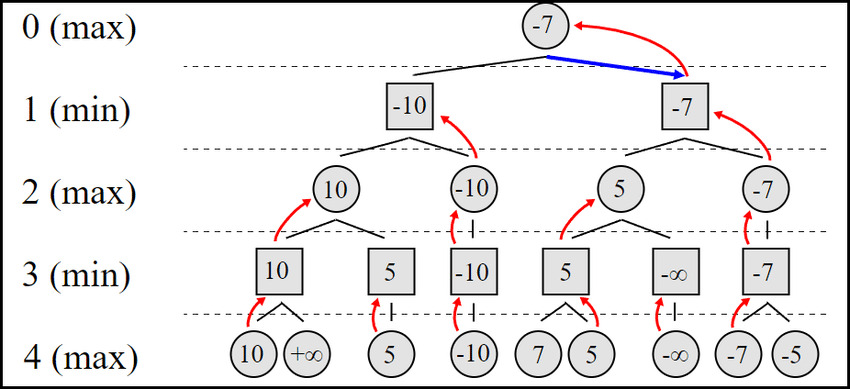
\includegraphics[width=0.75\textwidth]{MiniMax.jpg}}
    \caption{Algorithme Minimax et arbre de décision}\label{fig:minimax}
\end{figure}



La complexité exponentielle du Minimax l'oblige à explorer des branches dont le calcul s'avère en réalité inutile, l'élagage Alpha-Bêta permet précisément de les ignorer.



\subsubsection{Optimisation : L'Élagage Alpha-Bêta}

L'élagage Alpha-Bêta est l'optimisation mathématique de référence pour le Minimax. Cette technique réduit le nombre de nœuds à explorer en ignorant les branches qui ne peuvent pas aboutir à un meilleur score que celui déjà garanti par une autre branche. L'élagage maintient l'optimalité du résultat avec un gain de vitesse considérable.

L'exploration exhaustive de l'arbre de jeu étant trop coûteuse en ressources, l'algorithme maintient deux bornes de coupe (des limites mathématiques permettant de stopper prématurément le calcul) :

Afin de limiter la consommation de ressources lors d'une exploration exhaustive, l'algorithme maintient deux bornes de coupe essentielles : $\alpha$, représentant le score minimum garanti pour le joueur MAX (l'intelligence artificielle), et $\beta$, correspondant au score maximum garanti pour le joueur MIN (l'adversaire).
Durant la descente dans l'arbre, l'algorithme compare constamment les options des deux joueurs, et l'exploration d'une branche est immédiatement interrompue (élaguée) dès que la condition $\alpha \ge \beta$ est validée. Pour comprendre logiquement cette mécanique, il faut considérer la valeur $\alpha$ comme l'assurance de l'intelligence artificielle (le joueur MAX) : c'est le score minimum qu'elle s'est déjà garanti en explorant une branche précédente. Lorsque l'algorithme commence à évaluer une nouvelle alternative (un autre coup possible pour MAX), il simule les réponses de l'adversaire (le joueur MIN). Si, au cours de cette simulation, l'algorithme découvre un coup pour MIN qui fait chuter l'évaluation à une valeur $\beta$ inférieure ou égale à l'assurance $\alpha$, le calcul s'arrête. En effet, le but de MIN étant de minimiser le score, il choisira à coup sûr cette réponse punitive, ou une pire encore s'il en trouve une en cherchant plus loin. Anticipant cela, MAX sait pertinemment que s'engager dans cette direction le forcera à subir ce score $\beta$, ce qui est strictement moins avantageux que son plan de secours $\alpha$ déjà sécurisé ailleurs. MAX ne choisira donc jamais d'emprunter ce chemin initialement. Par conséquent, il devient mathématiquement inutile de gaspiller du temps de calcul pour évaluer le reste de la branche, justifiant ainsi la coupe immédiate du nœud.

Cette coupe radicale permet de dédier la puissance de calcul aux branches viables, augmentant mécaniquement la profondeur d'analyse dans la limite de temps impartie.


\subsubsection{L'Évaluation Heuristique : Le Moteur de Décision de l'IA}

Lorsqu'un nœud atteint la profondeur maximale ou que le temps est écoulé, la partie n'est généralement pas terminée. L'algorithme fait alors appel à une fonction d'évaluation (heuristique) pour estimer la valeur tactique de cette position précise. Plus ce score est élevé, plus la situation est jugée favorable pour l'IA (MAX). Le projet propose trois niveaux d'évaluation :

\paragraph{L'Heuristique Simple (SimpleHeuristic)}

L'Heuristique Simple (SimpleHeuristic) se concentre sur l'objectif le plus rudimentaire du jeu, qui est d’avancer vers l'arrivée. D'un point de vue théorique, elle s'appuie sur une évaluation spatiale purement absolue en calculant le nombre de cases franchies en ligne droite par rapport à sa position de départ. Bien que cette méthode arithmétique soit extrêmement rapide à calculer, elle présente des limites tactiques majeures : elle reste totalement ignorante de son environnement puisqu'elle ne prend en compte ni les murs posés sur le plateau, ni la position actuelle de l'adversaire, comme le proposait Mertens \cite{mertens2006}.

\paragraph{L'Heuristique Intermédiaire (MediumHeuristic)}

L'Heuristique Intermédiaire (MediumHeuristic) affine cette première approche en introduisant la notion d'avantage relatif. Plutôt que d'évaluer l'intelligence artificielle de manière isolée, elle reprend exactement la logique de l'heuristique simple et l'applique aux deux joueurs pour en extraire un différentiel. L'algorithme calcule le nombre de cases franchies en ligne droite par l'IA depuis sa position de départ, puis y soustrait cette même mesure effectuée pour l'adversaire. Cette évaluation reste strictement spatiale et calcule une distance directe, ignorant la présence éventuelle de murs sur le trajet. Un score positif indique ainsi clairement que l'IA est physiquement en tête de la course. Surtout, cette comparaison de distances incite naturellement l'algorithme à jouer de manière défensive. Si la pose d'un mur ralentit fortement la progression ennemie sans trop pénaliser celle de l'IA, l'écart mathématique entre les deux joueurs augmentera, validant ainsi la pertinence de ce blocage tactique.

\paragraph{L'Heuristique Avancée (AdvancedHeuristic)}

L'Heuristique Avancée (AdvancedHeuristic) constitue le véritable cerveau tactique du joueur Minimax. Elle calcule son score final en agrégeant plusieurs métriques dynamiques, c'est-à-dire des mesures chiffrées qui évoluent en temps réel selon la configuration du plateau, contrairement à des valeurs fixes. Ces métriques incluent l'analyse spatiale des obstacles, la gestion de la réserve de murs et la capacité à forcer des détours.

Tout d'abord, contrairement aux heuristiques précédentes basées sur des coordonnées brutes, elle effectue une analyse topographique concrète : elle étudie le relief du terrain créé par les murs. Elle calcule la vraie distance requise pour gagner en tenant compte du labyrinthe formé par les obstacles déjà posés, en utilisant l'algorithme de parcours en largeur BFS (Breadth-First Search). Ce dernier explore systématiquement toutes les cases accessibles pour garantir le calcul du chemin le plus court.

Ensuite, elle intègre une gestion des ressources en comparant le nombre de murs non joués restants dans la main de l'IA par rapport à ceux de l'adversaire. Cet avantage matériel est modulé par un coefficient fluctuant (wallCoeff). Ce coefficient traduit le fait qu'un mur conservé en réserve en début de partie rapporte beaucoup de points en raison de son fort potentiel de blocage, mais que sa valeur tactique (son utilité réelle pour gagner) diminue à mesure que l'IA approche de la victoire et que les opportunités de pose se raréfient.

Le cœur de cette heuristique repose sur la stratégie de contournement, c'est-à-dire l'art d'obliger l'adversaire à s'éloigner de son chemin le plus direct. Pour évaluer la réussite de cette stratégie, l'algorithme calcule un bonus de détour en comparant la distance théorique de l'adversaire sans aucun obstacle (la distance de Manhattan, qui est la somme des différences absolues de coordonnées) avec sa distance réelle trouvée par le parcours BFS. La différence entre ces deux valeurs représente le détour exact imposé par les murs placés sur le plateau. L'IA est ainsi lourdement récompensée (WALL\_BONUS) si elle parvient à créer des goulots d'étranglement obligeant l'adversaire à emprunter de longs chemins sinueux.

Enfin, l'algorithme gère les conditions de victoire de manière prioritaire pour éviter que des calculs secondaires ne masquent un gain ou une perte imminente. Dans l'implémentation, le seuil de victoire est une constante nommée WIN\_THRESHOLD fixée à la valeur 1, représentant la distance minimale, calculée en nombre de pas par l'algorithme BFS, séparant un pion de sa ligne d'arrivée. Ce seuil est déterminé dynamiquement à chaque évaluation : l'IA lance un parcours de graphe pour elle-même et pour son adversaire afin de connaître le nombre précis de cases restant à parcourir en tenant compte des murs. Si le résultat est inférieur ou égal à 1, cela signifie que le joueur est soit déjà sur sa ligne d'arrivée, soit à une seule case de celle-ci. Dès que cette proximité extrême est détectée, la fonction interrompt immédiatement l'agrégation des autres métriques, comme la réserve de murs ou les bonus de détour, car elles n'ont plus d'importance tactique face à une fin de partie immédiate. L'algorithme renvoie alors un score absolu de 10 000 pour une victoire de l'IA ou de -10 000 pour une victoire adverse, garantissant que l'intelligence artificielle privilégiera toujours le coup menant au succès final plutôt qu'une simple amélioration stratégique.


\paragraph{Structures de Données et Optimisations (Minimax)}

L'implémentation repose sur des structures de données spécifiquement choisies pour limiter l'empreinte mémoire (la quantité de mémoire vive RAM consommée) et accélérer la vitesse d'exécution :

Cette implémentation repose sur des structures de données optimisées : une file à double entrée (Deque) permet d'explorer l'arbre par mutation directe et backtracking sans clonage massif du plateau ; une table de hachage sécurisée (ConcurrentHashMap) assure une extraction thread-safe des paramètres internes pour l'interface graphique ; et des listes dynamiques (List) stockent les séquences de cases validées par l'algorithme BFS pour une évaluation heuristique précise.

\paragraph{L'Approfondissement Itératif (Iterative Deepening)}

Cet algorithme, plutôt que d'explorer l'arbre à une profondeur fixe définie arbitrairement, exécute des recherches successives à des profondeurs croissantes. Le principal atout de cette méthode est sa capacité à fournir une réponse optimale à tout moment. Si le temps alloué (reflexionTime) s'écoule pendant l'exploration de la profondeur $p$, l'algorithme interrompt le calcul et renvoie le meilleur coup identifié lors de l'itération à la profondeur $p-1$. Contrairement à Minimax qui, s'il est interrompu, fournit un résultat aléatoire, l'Iterative Deepening garantit une décision tactique basée sur l'exploration complète la plus profonde possible. Cette méthode introduit donc une stratégie de gestion dynamique de la profondeur de recherche qui vient compléter l'élagage Alpha-Bêta pour pallier l'imprévisibilité de la qualité du coup joué.

L’inconvénient de cette méthode réside dans la redondance : chaque nouvelle itération recommence l'exploration des premiers niveaux de l'arbre déjà parcourus. Cependant, dans un jeu comme le Quoridor où le facteur de branchement est important, ce surcoût reste acceptable car le temps recalculé pour une profondeur $p$ va représenter un temps de calcul très faible par rapport à celui de l'itération finale \cite{KORF198597}.


Bien que l'algorithme Minimax soit redoutable, son exploration systématique montre ses limites face à des situations présentant un fort facteur de branchement, où le nombre de coups possibles devient beaucoup trop grand pour être calculé dans le temps imparti. C'est pour pallier cette explosion combinatoire qu'intervient l'algorithme Monte Carlo Tree Search (MCTS).



\subparagraph{Mécanique de l'Algorithme Monte Carlo Tree Search}

Contrairement au Minimax qui tente d’évaluer toutes les éventualités, le MCTS ne vérifie pas toutes les possibilités. Il s’agit d’une approche probabiliste, signifiant qu’elle fait intervenir l’aléatoire dans ses choix de simulation, et asymétrique, car elle concentre sa puissance de calcul pour explorer en profondeur les branches les plus prometteuses plutôt que de parcourir l’arbre de manière uniforme\cite{browne2012mcts}. Le processus itératif s’exécute en boucle selon quatre phases distinctes orchestrées par la méthode getBestMoveAfterSearch dans la classe MctsNode (Fig.~\ref{fig:mcts}).

\begin{figure}[H]
    \centering
    \frame{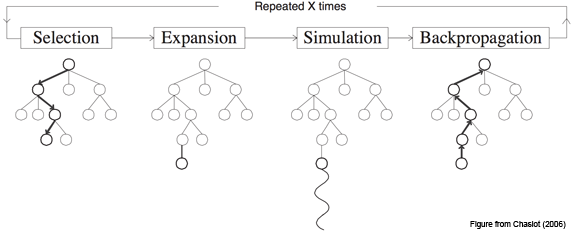
\includegraphics[width=0.75\textwidth]{mcts-algorithm-1a.png}}
    \caption{Les quatre phases de l'algorithme MCTS}\label{fig:mcts}
\end{figure}


La première phase est la sélection, étape au cours de laquelle l'algorithme amorce sa recherche en descendant dans l'arbre depuis la racine. Le but de cette descente est de trouver le candidat idéal pour poursuivre l'exploration. L'algorithme obéit à une règle de priorité stricte dictant le passage à l'étape suivante. En effet, tant qu'un état a déjà testé l'intégralité de ses coups possibles et possède des nœuds enfants, la phase de sélection continue de s'enfoncer dans l'arbre. À chaque intersection, l'intelligence artificielle choisit de descendre vers le nœud enfant le plus "prometteur", c'est-à-dire celui qui maximise le score évalué par la méthode bestUCT. Ce score prometteur désigne le meilleur compromis mathématique calculé entre l'exploitation d'une branche affichant déjà un fort taux de victoire et l'exploration nécessaire des chemins encore peu visités, principe fondamental du MCTS\cite{browne2012mcts}.

Cependant, dès que l'algorithme croise au cours de sa descente un nœud disposant encore d'au moins un coup légal non essayé (une condition vérifiée dynamiquement par la méthode hasUntriedLegalMoves), la phase de sélection s'arrête net. Ce nœud partiellement exploré devient alors la cible prioritaire absolue pour la phase suivante, garantissant ainsi que l'arbre s'élargisse systématiquement pour évaluer toutes les options initiales d'une position avant de se creuser aveuglément en profondeur.

Vient ensuite la phase d'expansion. Si le nœud sélectionné n'est pas un état de fin de partie, un coup non testé est extrait pour créer un nouveau nœud enfant dans l'arbre de recherche. Pour implémenter cela efficacement, la classe MctsNode s'appuie sur des listes dynamiques. Lors de sa création, chaque état génère et stocke ses coups potentiels dans une liste dédiée nommée untriedMoves. Afin de garantir la stochasticité de l'algorithme\label{sec:stochasticite}, c'est-à-dire l'introduction d'un hasard mathématique visant à neutraliser l'ordre prévisible dans lequel le jeu génère initialement les actions, cette collection est immédiatement mélangée grâce à la fonction Collections.shuffle\cite{browne2012mcts}.

Une optimisation majeure de cette phase d'expansion réside dans la vérification paresseuse des coups. Dans un jeu comme Quoridor, calculer la légalité absolue de toutes les poses de murs possibles est extrêmement lourd en ressources. Pour éviter ce goulet d'étranglement, la création du nœud génère uniquement des coups dits "pseudo-légaux". Ce type d’optimisation est couramment utilisé dans les implémentations pratiques du MCTS\cite{browne2012mcts}.


Dans le cas contraire, si l'expansion aboutit à un état en cours de jeu, l'algorithme enclenche la troisième phase : la simulation (Playout). À partir de ce nouveau nœud, l'algorithme simule une fin de partie en jouant une série de déplacements aléatoires jusqu'à déterminer un vainqueur.

Enfin, la rétropropagation (Backpropagation) clôture le cycle en remontant le résultat de cette simulation le long de la branche explorée afin de mettre à jour les statistiques des nœuds parents. Chaque nœud conserve un nombre de visites et un nombre de victoires. Ces valeurs permettent de calculer le taux de victoire utilisé dans la formule UCT pour guider les futures explorations.

\subparagraph{Exploration et Exploitation : Le Calcul UCT}

La véritable intelligence du MCTS réside dans sa phase de sélection, pilotée par la classe MctsPlayer. Bien que cette classe puisse dynamiquement déléguer ce choix à un réseau de neurones artificiels (une approche détaillée dans la section suivante), nous nous concentrerons ici sur sa méthode d'évaluation classique nommée selectBestChildUsingUCT. Pour choisir le chemin à emprunter dans l'arbre, l'algorithme utilise la formule mathématique UCT (Upper Confidence bounds applied to Trees). Cette équation garantit un compromis rigoureux entre l'exploitation et l'exploration.

Mathématiquement, l'algorithme calcule pour chaque nœud enfant un score composé de deux parties. La première partie est le taux de victoire brut, obtenu en divisant le nombre de victoires par le nombre de visites de ce nœud. Cela représente l'exploitation, signifiant concrètement le fait de privilégier les coups ayant déjà prouvé leur efficacité. La seconde partie est le terme d'exploration, calculé en multipliant une constante fixée à 1.41 par la racine carrée du logarithme des visites du nœud parent divisé par les visites de l'enfant. Ce terme d'exploration augmente artificiellement le score des branches qui ont été peu visitées. Ainsi, l'algorithme est naturellement poussé à vérifier les coups ignorés pour s'assurer de ne rater aucune stratégie cachée, tout en continuant d'approfondir les lignes de jeu majoritairement gagnantes.



\subparagraph{Les Limites de la Simulation Aléatoire et l'Introduction au Machine Learning}

Si la méthode UCT standard est très performante pour diriger la recherche, elle repose fondamentalement sur la phase de simulation (le Playout aléatoire) pour évaluer la qualité d'un nœud. Dans un jeu complexe, jouer des coups au hasard jusqu'à la fin de la partie peut aboutir à des résultats chaotiques qui ne reflètent pas la véritable valeur stratégique d'une position. Un simple mur placé au hasard peut fausser toute l'évaluation. Pour pallier cette limite, l'intelligence artificielle introduit un modèle d'apprentissage automatique supervisé, une architecture héritée des travaux révolutionnaires d'AlphaZero combinant recherche arborescente et évaluation neuronale\cite{silver2017masteringchessshogiselfplay}. La classe \texttt{MctsPlayer} agit alors comme un aiguilleur paramétrable offrant la possibilité de configurer le moteur de recherche selon deux modes exclusifs, c'est-à-dire en utilisant soit l'approche UCT traditionnelle, soit le réseau de neurones. Lorsque l'apprentissage automatique est sélectionné, le modèle neuronal évalue instantanément les chances de victoire de la position en cours au lieu de se fier au calcul mathématique classique. Cette approche remplace ainsi avantageusement la dépendance à la lourde phase de simulation aléatoire par une prédiction déterministe et stratégiquement éclairée. Le terme déterministe certifie que pour une configuration strictement identique du plateau, le réseau de neurones renverra toujours exactement le même score de victoire, puisqu'il remplace le hasard des simulations par un calcul matriciel aux paramètres fixes. Parallèlement, cette prédiction est qualifiée de stratégiquement éclairée car elle ne se base plus sur des déplacements effectués à l'aveugle. Le modèle analyse concrètement la qualité de la position en évaluant la véritable distance séparant les joueurs de leur ligne d'arrivée et en comptabilisant le nombre de murs restants dans les réserves, appliquant ainsi une réelle compréhension tactique acquise lors de son entraînement.

\subparagraph{L'Architecture du Neurone et la Gestion des Tenseurs}

L'évaluation neuronale est encapsulée dans la classe NeuralNetworkEvaluator, qui sert d'interface avec le moteur de calcul TensorFlow. Ce modèle s'appuie spécifiquement sur une architecture de type régression logistique, ce qui correspond structurellement à l'utilisation d'un unique neurone artificiel.

Le fonctionnement de ce neurone repose sur une équation mathématique fondamentale où la prédiction finale est le résultat de l'opération $P = \sigma(W \cdot X + b)$ (Fig.~\ref{fig:neurone}). Dans cette formule, la variable $X$ représente les caractéristiques en entrée fournies par le jeu. La variable $W$ désigne les poids de la matrice, représentant l'importance accordée par l'intelligence artificielle à chaque paramètre. Enfin, la variable $b$ correspond au biais, un ajustement numérique global indépendant des entrées.

\begin{figure}[H]
    \centering
    \frame{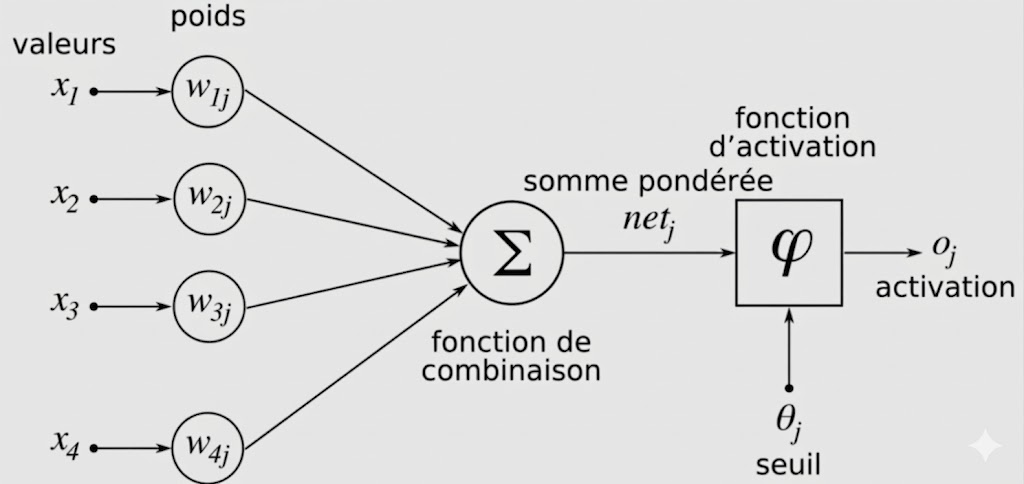
\includegraphics[width=0.8\textwidth]{Neurone_4_poids.jpeg}}
    \caption{Modèle de neurone artificiel pour l'évaluation}\label{fig:neurone}
\end{figure}


Le système prend en entrée quatre caractéristiques mathématiques précises extraites de la partie en cours. Il calcule d'abord la véritable distance séparant le joueur de sa ligne d'arrivée en effectuant un parcours de graphe BFS. Pour que cette donnée soit exploitable par le réseau de neurones, elle doit être normalisée. L'algorithme divise donc ce nombre de pas par la distance maximale théorique du plateau, puis inverse mathématiquement ce résultat. Ainsi, une distance nulle produit la valeur maximale de 1.0 pour indiquer une victoire atteinte, tandis que l'éloignement maximal donne un résultat de 0.0. Il intègre ensuite la distance de l'adversaire, elle aussi obtenue par un algorithme BFS et divisée par la distance maximale. Il est important de noter que cette valeur adverse n'est pas inversée, car pour l'intelligence artificielle, un résultat de 1.0 indiquant que l'ennemi est bloqué très loin constitue une situation hautement favorable. Les troisième et quatrième paramètres sont respectivement le nombre de murs restants pour l'IA et pour son adversaire, tous deux divisés par leur capacité initiale de dix (si la capacité initiale est supérieure à 10, on s’assure de rester dans l'intervalle [0,1] en prenant 1.0 au maximum) . Cette dernière opération permet de ramener l'intégralité des données fournies au neurone sur une échelle mathématique parfaitement homogène comprise entre zéro et un.

L'algorithme de TensorFlow applique alors une multiplication matricielle entre ces quatre entrées $X$ et leurs poids respectifs $W$, additionne le biais $b$, puis fait passer le résultat brut par la fonction d'activation sigmoïde désignée par le symbole $\sigma$. Cette fonction prend la forme d'une courbe en "S" écrasant les valeurs numériques pour forcer un résultat strictement compris entre 0 et 1, représentant ainsi de façon lisible le pourcentage direct de chances de victoire de la position évaluée.

Techniquement, pour interagir avec le cœur natif de TensorFlow, les données primitives Java sont systématiquement converties en tenseurs de type TFloat32. Ce sont des matrices multidimensionnelles hautement optimisées pour être manipulées très rapidement par le moteur C++ sous-jacent. De plus, le graphe computationnel modélisant ces opérations mathématiques et la session d'exécution sont maintenus ouverts en mémoire vive. Cette architecture évite le coût de latence massif qu'impliquerait une recompilation du modèle à chaque nouvelle inférence requise par le MCTS. Pour gérer rigoureusement ces ressources externes, la classe implémente l'interface native AutoCloseable. Cette sécurité garantit la destruction explicite des objets alloués en C++ à la fermeture du programme, prévenant toute fuite de mémoire (Memory Leak) puisque ces objets échappent par nature au ramasse-miettes (Garbage Collector) de Java.

\subparagraph{L'Entraînement Supervisé et la Descente de Gradient}

Pour que ce neurone artificiel et ses poids internes soient capables d'évaluer correctement une position, il faut d'abord les ajuster lors d'une phase d'apprentissage autonome. La classe NeuralNetworkTrainer est responsable de cet entraînement supervisé. Elle génère d'énormes quantités de données en faisant s'affronter l'IA contre elle-même (Self-Play) au travers de milliers de parties simulées. Durant ces simulations de génération de données, l'algorithme applique une politique d'exploration appelée Epsilon-Greedy. Une probabilité fixée à dix pour cent force ponctuellement l'IA à jouer des coups totalement aléatoires. Le reste du temps, le système ne cherche pas à calculer le meilleur mouvement tactique absolu de la position, mais délègue plutôt la décision à un algorithme Minimax intentionnellement bridé à une profondeur de recherche d'un seul tour. Ce choix technique est un compromis indispensable pour garantir la rapidité des simulations, puisqu'une recherche complète et profonde prendrait un temps incalculable pour générer les milliers de parties requises par l'apprentissage. Cette mécanique hybride empêche finalement l'algorithme de tourner en boucle sur les mêmes séquences d'ouverture et le force à découvrir de nouvelles configurations complexes du labyrinthe tout en générant des données de jeu cohérentes.

Une fois ces parties terminées et les résultats finaux connus, le réseau compare ses propres prédictions passées avec la réalité des victoires et des défaites. Cette différence est mesurée avec une grande précision par une fonction mathématique nommée Entropie Croisée Binaire, ou Binary Crossentropy. Cette fonction de perte calcule l'écart entre la probabilité prédite par la sigmoïde et le label réel de la partie, valant 1.0 pour une victoire observée et 0.0 pour une défaite. La particularité mathématique de l'Entropie Croisée Binaire est d'appliquer une pénalité logarithmique extrêmement sévère si le modèle se trompe en étant très confiant, par exemple s'il prédisait 90 pour cent de chances de victoire pour une position qui a finalement mené à un échec.

Afin de corriger cette erreur de prédiction, l'algorithme fait appel à un optimiseur basé sur la méthode de la Descente de Gradient. Ce mécanisme mathématique calcule la dérivée de l'erreur pour déterminer dans quelle direction modifier les variables internes. Il ajuste alors de manière infime les poids synaptiques $W$ et le biais $b$ du neurone en fonction d'un taux d'apprentissage défini, afin que lors de la prochaine situation similaire, la prédiction se rapproche naturellement de la réalité. En répétant ce cycle d'évaluation et de correction sur des dizaines de milliers d'exemples répartis sur plusieurs centaines d'époques d'entraînement, le modèle met progressivement à jour sa matrice de poids pour affiner sa compréhension tactique du jeu.





\newpage
\section{Architecture du projet}

Notre projet  consiste à implémenter le jeu Quoridor en Java, en respectant strictement l’ensemble des règles détaillées
dans la section précédente « Les règles du jeu ». Au-delà de la simple reproduction des mécaniques, notre cahier des charges
impose plusieurs contraintes et objectifs qui influencent directement le choix de l’architecture logicielle.
En particulier, nous devons intégrer trois modes d’interaction distincts : le mode en ligne de commande (CLI),
une interface graphique (GUI) et un mode réseau permettant de jouer avec d’autres utilisateurs à distance.
À cela s’ajoutent des exigences concernant l’intelligence artificielle : le système doit pouvoir exécuter plusieurs algorithmes,
notamment Minimax et Monte Carlo Tree Search (MCTS), pour simuler des adversaires compétitifs et variés.

Pour répondre efficacement à ces besoins complexes, nous avons choisi une architecture modulaire orientée domaine,
inspirée de la Clean Architecture telle que décrite par Martin\cite{martin2017clean}. Cette décision repose sur plusieurs
considérations pratiques et théoriques, toutes centrées sur la nécessité de séparer clairement les responsabilités et
de rendre notre application à la fois extensible, maintenable et testable.

\subsection{Explication en profondeur de l’Architecture }

\paragraph{Principes fondamentaux de la Clean Architecture}

La Clean Architecture repose sur un principe central : la séparation stricte entre la logique métier et les détails techniques
de l’implémentation. Dans notre contexte, cela signifie que toutes les règles et entités du jeu — pions, murs, plateaux, mouvements,
validation des coups, état de la partie — sont encapsulées dans un cœur métier indépendant de toute interface utilisateur,
du réseau ou de l’intelligence artificielle. Ce cœur, que nous avons regroupé dans le package \texttt{Core}, contient toutes
les entités et services nécessaires au fonctionnement du jeu. Il ne connaît rien des mécanismes de présentation, de stockage
ou de communication, ce qui garantit que la logique métier reste cohérente et isolée.

Cette approche est cohérente avec les recommandations de Fowler\cite{fowler2002patterns} sur les patterns d’architecture logicielle.
Fowler insiste sur la nécessité de séparer les préoccupations et de structurer les systèmes en couches bien définies, afin de réduire
les dépendances entre les composants et de faciliter la maintenance.
En suivant ce principe, notre architecture repose sur quatre couches concentriques clairement identifiées : la \textbf{Lancement et Initialisation (\texttt{L1})} qui regroupe le mode de démarrage (\texttt{main}) et les interfaces utilisateur ; les \textbf{Adaptateurs applicatifs (\texttt{L2})} incluant l'intelligence artificielle et la persistance ; le \textbf{Support Domaine (\texttt{L3})} fournissant les services techniques comme le logging et la traduction ; et enfin le \textbf{centre du système (\texttt{L4})} constitué du cœur métier pur (\texttt{Core} et \texttt{Graph}).

\paragraph{Avantages pratiques de cette approche}

L’un des principaux avantages de cette architecture est sa modularité. Elle permet de développer et tester chaque composant indépendamment, les tests unitaires pouvant se focaliser sur le cœur métier sans dépendances. Elle offre également la flexibilité d'ajouter des fonctionnalités (comme une version mobile) sans impacter l'existant, et facilite l'introduction de nouveaux algorithmes d'IA qui sollicitent simplement le cœur via des interfaces.

Un autre avantage majeur réside dans la robustesse et la sécurité fonctionnelle. Toutes les actions initiées par un joueur ou par un algorithme passent par le cœur métier pour validation. Cela signifie qu’aucune interface ne peut créer d’état invalide : impossible de poser un mur illégal, de déplacer un pion hors du plateau ou de contourner les règles fondamentales. Cette approche centralise la logique critique et prévient les bugs liés à des incohérences entre différents modules.

\paragraph{Interaction entre couches et adaptateurs}

Les adaptateurs constituent le lien entre le monde extérieur et le cœur métier via des interfaces abstraites. La CLI interprète les commandes terminal pour \texttt{GameEngine}, tandis que la GUI gère les interactions graphiques. Le module réseau synchronise les actions distantes avec le cœur, et les modules d'IA génèrent les meilleurs coups en analysant l'état du plateau.

Cette conception permet à chaque adaptateur de se concentrer sur ses responsabilités spécifiques sans se soucier des règles métier, tout en assurant une cohérence globale du système.

\paragraph{Testabilité et maintenance}

L’un des aspects les plus valorisés de cette architecture est sa testabilité. Le cœur métier peut être testé en isolation complète, ce qui permet de vérifier toutes les règles du jeu, la gestion des murs, la détection de victoire et les comportements spécifiques sans dépendre de l’interface graphique ou du réseau. Cela réduit considérablement les risques d’erreurs et simplifie la détection de bugs.

De plus, la maintenance est facilitée. Si, à l’avenir, nous souhaitons modifier l’interface graphique ou ajouter un mode de jeu supplémentaire, aucune modification n’est nécessaire dans le cœur métier. Les interfaces sont découplées, ce qui signifie que les changements techniques ou esthétiques ne perturbent pas la logique fondamentale du jeu. Cette modularité garantit également une meilleure évolutivité à long terme : le projet peut croître et intégrer de nouvelles fonctionnalités sans remettre en cause les composants existants.

\paragraph{Flexibilité pour les algorithmes d’intelligence artificielle}

Dans le cadre de notre projet, la Clean Architecture est particulièrement adaptée à l’intégration d’algorithmes d’IA, permettant d’implémenter indépendamment \textbf{Minimax} pour une évaluation systématique par arbre de décision, et \textbf{Monte Carlo Tree Search (MCTS)} pour une exploration probabiliste des stratégies prometteuses.

Chaque algorithme interagit uniquement avec le cœur métier via des interfaces abstraites, ce qui permet d’ajouter ou de remplacer un algorithme sans modifier la logique du jeu. Par exemple, nous pourrions expérimenter un nouvel algorithme hybride combinant MCTS et Minimax, ou encore intégrer des techniques d’apprentissage automatique pour améliorer les performances de l’IA, sans toucher au reste de l’architecture.

\paragraph{}

En résumé, le choix d’une architecture modulaire orientée domaine, inspirée de la Clean Architecture\cite{martin2017clean},
se justifie pleinement par les besoins spécifiques de notre projet Quoridor. Elle garantit la cohérence de la logique métier,
facilite l’intégration de multiples interfaces, permet l’ajout et le test d’algorithmes d’intelligence artificielle variés,
et assure une maintenance et une évolutivité sur le long terme. L’adoption des principes de séparation des responsabilités
et de structuration en couches, également recommandée par Fowler\cite{fowler2002patterns}, renforce cette cohérence et permet
de construire un système robuste, flexible et modulaire, capable de répondre à tous les objectifs fonctionnels et techniques
définis dans notre cahier des charges.

\subsection{Vue d'ensemble des packages}

Cette organisation en packages nous permet de structurer le projet de manière claire et cohérente. Chaque package a un rôle précis, ce qui favorise la modularité, la testabilité et la maintenance du code dans notre projet. De plus, elle nous facilite l’ajout futur de fonctionnalités, qu’il s’agisse d’IA avancées, de nouvelles interfaces ou de modes de jeu supplémentaires, tout en garantissant la robustesse et la cohérence des règles de Quoridor.

Voici les onze packages distincts de notre projet, chacun ayant une responsabilité bien définie que nous décrivons ici :


\begin{table}[H]
\centering
\begin{tabular}{|p{2cm}|p{13cm}|}
    \hline
    \textbf{Package} & \textbf{Responsabilité} \\
    \hline
    core & constitue le cœur métier de l’application. Il regroupe toutes les entités fondamentales du jeu,
    telles que \texttt{Board} pour représenter le plateau, \texttt{GameState} pour l’état général de la partie,
    \texttt{Player} pour les joueurs, \texttt{Move} pour les déplacements, \texttt{Position} pour la localisation des pions,
    ainsi que \texttt{GameEngine} et \texttt{RuleChecker} pour gérer les règles et la logique de progression du jeu.
    Ce package est totalement indépendant des interfaces graphiques, de la ligne de commande ou des modules réseau,
    ce qui garantit que toutes les règles sont appliquées de manière cohérente, quel que soit le mode de jeu choisi. \\
    \hline
    main & contient le point d’entrée de l’application. Il est responsable de la résolution du mode de lancement,
    que ce soit en CLI, en GUI ou en réseau, et applique le patron \textit{Factory} pour initialiser les composants
    nécessaires selon le contexte. Cette centralisation du lancement permet de simplifier la configuration initiale
    et de garantir que tous les modules sont correctement instanciés avant le démarrage de la partie. \\
    \hline
    cli & gère l’interface en ligne de commande. Il utilise le pattern \textit{Command} pour représenter chaque action que l’utilisateur peut effectuer, qu’il s’agisse de déplacer un pion, de poser un mur ou de demander l’aide. Ce design permet de découpler les commandes de l’exécution effective et de faciliter l’ajout de nouvelles commandes sans modifier la logique existante. \\
    \hline
    gui & basé sur JavaFX, implémente l’interface graphique. Il propose des menus principaux tels que \texttt{File} et \texttt{Game}, et permet à l’utilisateur de définir ses propres raccourcis clavier pour chaque action. Cette flexibilité améliore l’expérience utilisateur et rend l’interface plus ergonomique, tout en séparant la présentation de la logique métier contenue dans le package \texttt{core}.\\
    \hline
    network & est dédié à la gestion des fonctionnalités réseau. Il implémente un serveur TCP capable de gérer plusieurs clients simultanément, soit via un thread par client, soit par programmation asynchrone. Il intègre également une découverte UDP pour faciliter la connexion automatique des clients au serveur. Ce package assure la communication entre joueurs distants et garantit que toutes les actions reçues sont validées par le cœur métier. \\
    \hline
    ai & regroupe les différentes intelligences artificielles implémentées dans le projet. Il inclut des IA simples aléatoires, des IA basées sur Minimax avec élagage alpha-bêta et \textit{iterative deepening}, des IA utilisant Monte Carlo Tree Search, et des prototypes utilisant des réseaux de neurones. Ce package interagit uniquement avec le cœur métier via des interfaces abstraites, permettant d’échanger ou d’ajouter de nouveaux algorithmes facilement. \\
    \hline
    persistence & s’occupe de la sérialisation et désérialisation de l’état de jeu vers un fichier texte. Il assure que l’utilisateur peut sauvegarder et recharger une partie à tout moment, en conservant la cohérence des données avec le cœur métier. \\
    \hline
    util & contient des outils généraux, dont un \textit{Logger} singleton utilisé par l’ensemble de l’application pour tracer les actions, les erreurs et les événements importants, facilitant ainsi le débogage et la maintenance. \\
    \hline
    i18n & gère  la langue du logiciel. Il détecte automatiquement les variables d’environnement \texttt{LANG} ou \texttt{LC\_ALL} pour déterminer la langue par défaut, et permet d’adapter l’affichage et les messages aux préférences de l’utilisateur. \\
    \hline
    graph & fournit une représentation du plateau sous forme de graphe, avec une liste d’adjacence. Il contient le \texttt{GraphBuilder} qui permet de modéliser dynamiquement les mouvements possibles et les blocages liés aux murs, facilitant ainsi les calculs pour les IA et la validation des coups. \\
    \hline
    config & s’occupe de la configuration globale du logiciel. Il lit un fichier \texttt{.quoridorrc} situé dans le répertoire personnel de l’utilisateur (HOME) pour appliquer les options par défaut. Si le fichier est absent, un fichier minimal est créé automatiquement. Ce package centralise toutes les préférences, évitant la duplication de la configuration dans différents modules. \\
    \hline
\end{tabular}
\caption{Vue d'ensemble des packages}
\label{tab:packages}
\end{table}



\subsection{Vue de l'architecture en couches concentriques}

Dans cette section, nous présentons notre architecture structurée en quatre couches concentriques, où les dépendances pointent exclusivement vers l'intérieur pour préserver l'intégrité du domaine. 

\textbf{Couche 1 : Points d'Entrée et Lancement.} Elle regroupe les packages \texttt{main}, \texttt{gui}, \texttt{cli} et \texttt{network}. Cette couche est responsable de la capture des intentions de l'utilisateur ou des événements réseaux pour les transmettre aux couches plus profondes.

\textbf{Couche 2 : Adaptateurs Applicatifs.} Elle comprend les packages \texttt{ai}, \texttt{persistence} et \texttt{config}. Elle traduit les besoins de l'application (sauvegarde, intelligence artificielle, options de configuration) en actions sur le domaine.

\textbf{Couche 3 : Support et Infrastructure de Domaine.} Elle intègre \texttt{i18n} et \texttt{util}. Ces modules fournissent des services de traduction et de journalisation au Domaine via un mécanisme d'inversion de dépendance.

\textbf{Couche 4 : Centre du Domaine.} C'est le cœur du système composé de \texttt{core} et \texttt{graph}. Ce centre ne possède aucune dépendance vers l'extérieur et contient l'intégralité des règles métier.

Schéma en couches concentriques de notre architecture du projet (Fig.~\ref{fig:example1}).
\begin{figure}[H]
    \centering
    \frame{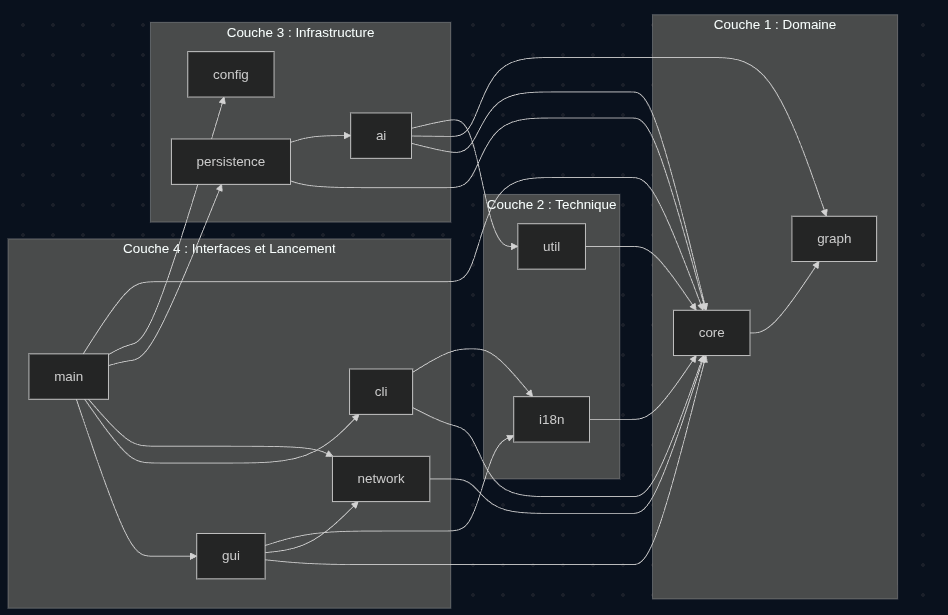
\includegraphics[width=1\textwidth]{quoridor}}
    \caption{Une architecture en couches concentriques}\label{fig:example1}
\end{figure}


\subsection{Couche Domaine --- Package \texttt{core}}

Le module \textbf{core} est le cœur du système. Il encapsule l'intégralité de la logique
métier du jeu et n'a aucune dépendance externe. Le \textbf{RuleChecker}
appelle le module \textbf{graph} pour vérifier qu'après la pose d'un mur, chaque joueur dispose encore
d'un chemin vers son bord cible.

Voici un diagramme indiquant comment sont liées les différentes classes du package Core.

Schéma de la couche Core de notre architecture (Fig.~\ref{fig:example0}).
\begin{figure}[H]
    \centering
    \frame{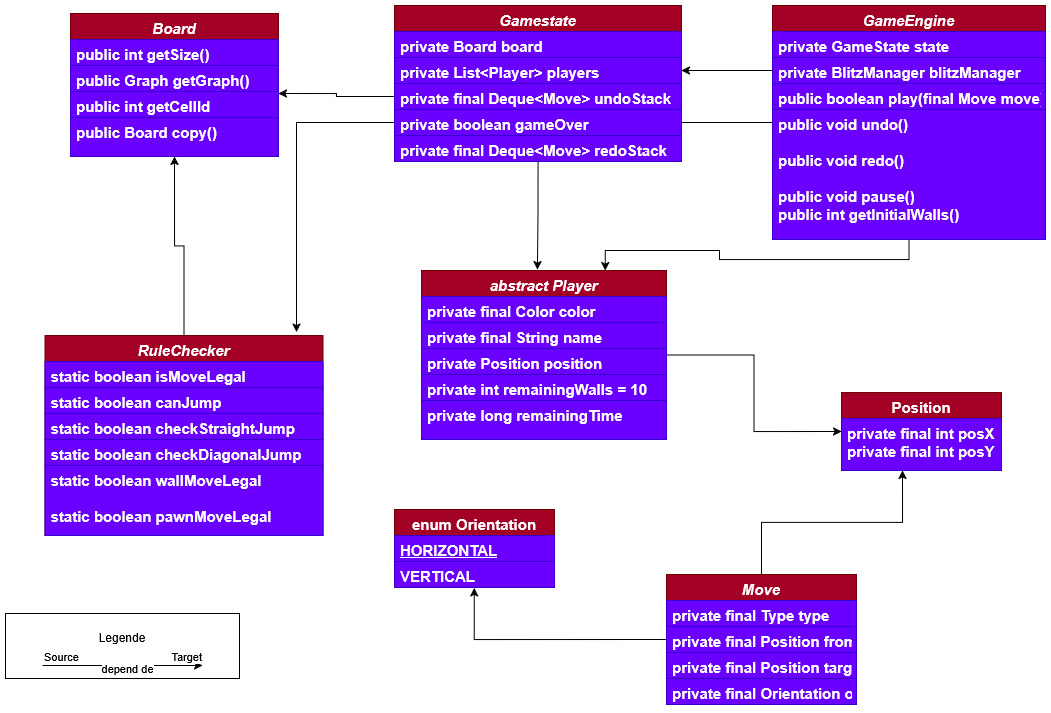
\includegraphics[width=0.75\textwidth]{core.jpg}}
    \caption{Le cœur métier (Core)}\label{fig:example0}
\end{figure}

\subsection{Couche Principale --- Package \texttt{Main}}
Le module \textbf{Main} joue le rôle de \textbf{composition root}
: il instancie tous les autres modules et câble leurs dépendances. Il utilise le pattern \textbf{Factory}
via \textit{AppLauncher} pour créer les adaptateurs selon le mode de lancement.

Au démarrage, le Main lit la configuration (.quoridorrc) pour déterminer le mode de jeu. Il instancie network si une partie réseau est demandée, gui pour le
mode graphique, cli pour le mode terminal. Il injecte les dépendances dans chaque module sans que ceux-ci se connaissent mutuellement.

Voici un diagramme indiquant comment sont liées les différentes classes du package Main.

Schéma de la couche Main de notre architecture (Fig.~\ref{fig:example2}).
\begin{figure}[H]
    \centering
    \frame{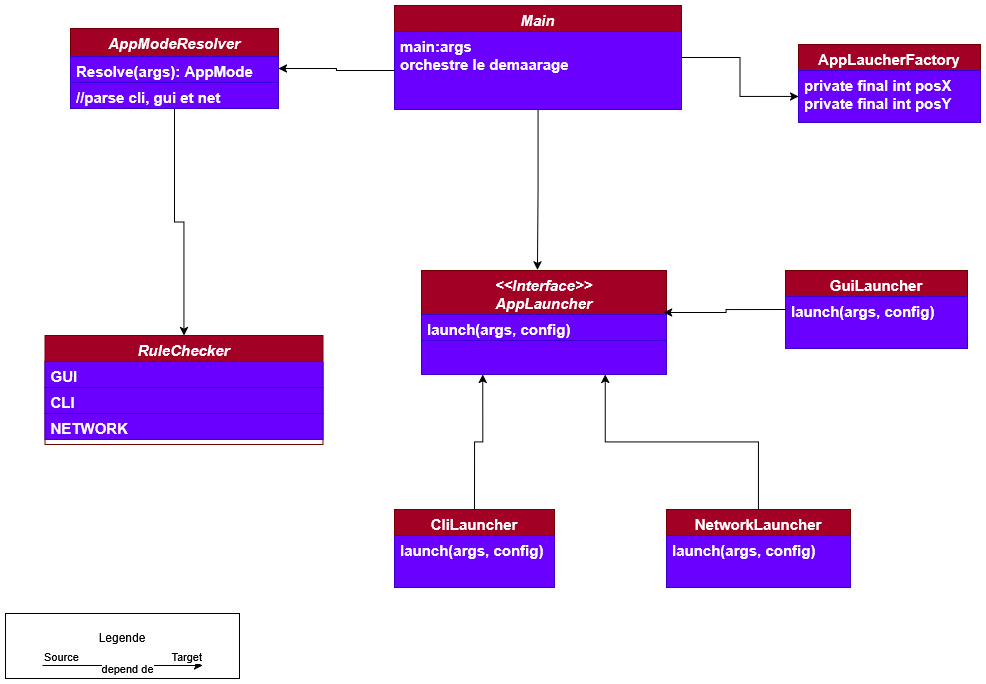
\includegraphics[width=0.75\textwidth]{main.jpg}}
    \caption{Couche Principale (Main)}\label{fig:example2}
\end{figure}

\subsection{Interface CLI --- Pattern Command}
Le module \textbf{cli} implémente le pattern \textbf{Command}
: chaque commande saisie est encapsulée dans un objet qui connaît son
action et peut être annulée. Ce pattern est adapté à Quoridor car il
permet de rejouer ou d'annuler l'historique des coups. Notre CLI est instanciée par Main au même titre que GUI et Network. Il lit les
entrées console, les analyse (parse), construit les objets Command correspondants et les exécute sur \textit{GameEngine}.
Le plateau est affiché en ASCII sur la sortie standard.

Voici un diagramme indiquant comment sont liées les différentes classes du package CLI.


schema du couche cli de notre architecture (Fig.~\ref{fig:example3}).
\begin{figure}[H]
    \centering
    \frame{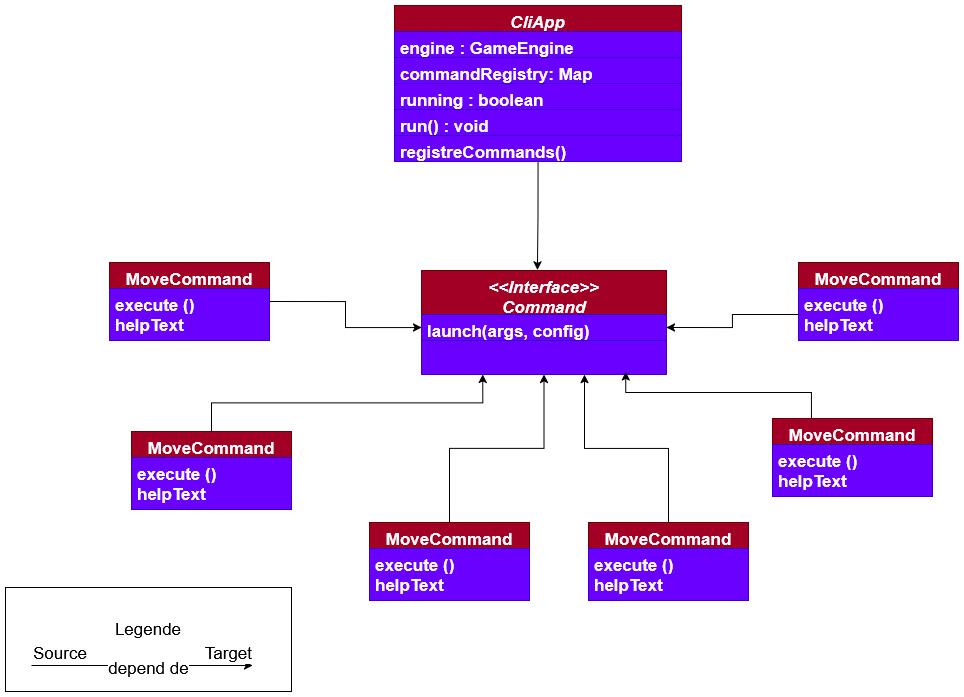
\includegraphics[width=0.75\textwidth]{cli.jpg}}
    \caption{Couche CLI}\label{fig:example3}
\end{figure}

\newpage
\section{Revue critique du projet}

Cette section propose un bilan analytique du projet, en examinant les succès techniques, les limites rencontrées lors du développement et les perspectives d'évolution pour le futur.

\subsection{Bilan des réalisations}

Le projet a atteint la grande majorité des objectifs fixés initialement. Toutes les fonctionnalités fondamentales (F1 à F11) liées à la gestion du jeu, à la validation des coups et à l'arbitrage automatique sont pleinement opérationnelles. Les interfaces CLI et GUI (JavaFX) offrent une expérience utilisateur fluide, intégrant la gestion des configurations ($F2$), l'internationalisation ($F3$) et le support du mode Blitz ($F5$). 

Sur le plan technique, l'implémentation des algorithmes d'IA (Minimax avec élagage alpha-bêta, MCTS et prototypes ML) constitue un succès majeur, tout comme le serveur réseau multi-clients ($F38$, $F39$). Seul le système avancé d'invitations (F40) reste partiellement réalisé, la découverte automatique des serveurs via UDP étant parfois limitée par les configurations réseaux spécifiques.

\subsection{Performances et cas limites}

L'utilisation d'une structure de graphe avec listes d'adjacence pour modéliser le plateau permet des calculs de chemin extrêmement rapides (via BFS), garantissant que la validation de la pose d'un mur reste imperceptible pour l'utilisateur.

En termes d'IA, l'algorithme Minimax combiné à l'approfondissement itératif (\emph{iterative deepening}\cite{KORF198597}) parvient à explorer l'arbre de jeu jusqu'à une profondeur de 4 à 6 niveaux dans le temps imparti de 5 secondes sur un matériel standard. Cependant, sur des plateaux de taille maximale ($15 \times 15$), le facteur de branchement élevé limite l'IA Minimax, rendant l'approche MCTS plus pertinente grâce à sa gestion probabiliste de l'exploration.

Les cas limites, tels que la pose d'un mur visant à enfermer totalement un joueur, sont systématiquement détectés et empêchés par le \texttt{RuleChecker}, assurant qu'au moins un chemin vers l'objectif reste toujours disponible, conformément aux règles officielles.

\subsection{Limitations et bugs connus}

Malgré une architecture robuste, certaines limitations techniques subsistent. Tout d'abord, le mécanisme de découverte réseau repose sur un protocole \emph{UDP broadcast} qui, bien qu'efficace sur un réseau domestique standard, peut présenter des défaillances sur des infrastructures plus complexes ou des réseaux locaux restreints par des pare-feux. Concernant l'interface graphique, bien que parfaitement fonctionnelle pour le mode classique, l'initialisation de parties à quatre joueurs via le menu réseau a révélé des temps de latence dans la synchronisation initiale de l'état du plateau, nécessitant une optimisation future. Enfin, le prototype basé sur l'apprentissage automatique constitue une avancée encourageante mais souffre encore d'un manque de généralisation. Pour rivaliser pleinement avec le moteur MCTS sur des configurations de plateau atypiques, le modèle nécessiterait un corpus de données d'entraînement beaucoup plus vaste et varié.

\subsection{Améliorations possibles}

Pour faire évoluer ce projet vers une version encore plus aboutie, plusieurs pistes de développement sont envisageables. La priorité résiderait dans la finalisation d'un système de salon de jeu complet, permettant une gestion fluide des invitations et des tournois en ligne. Sur le plan algorithmique, l'intégration de corpus de données issus de parties réelles jouées par des experts constituerait une avancée majeure pour affiner le modèle neuronal. Actuellement basé sur un entraînement par auto-jeu (self-play) incluant une part de coups aléatoires pour l'exploration, le système pourrait gagner en précision tactique en s'appuyant sur des séquences de jeu de haut niveau dépourvues de toute stochasticité artificielle (définie précédemment à la Section \ref{sec:stochasticite}). Cette approche permettrait à l'intelligence artificielle d'acquérir une compréhension plus profonde des ouvertures classiques et des stratégies de blocage complexes rencontrées dans les compétitions. Une autre évolution majeure consisterait à enrichir l'expérience utilisateur en passant d'une représentation bidimensionnelle à un moteur de rendu en trois dimensions, offrant une immersion accrue dans l'espace de jeu. Enfin, la portabilité du logiciel pourrait être étendue par l'adaptation de l'interface graphique pour les plateformes mobiles nativement, ou via une exportation vers le web, afin de rendre Quoridor accessible sur un plus large éventail de terminaux.

\subsection{IA utilisées}

Durant ce projet, nous avons utilisé certaines IAs pour nous aider, notamment pour la génération de code, la correction de bugs, et l'amélioration de notre code. L'utilisation de ces outils s'est faite de manière raisonnée, c'est-à-dire qu'on a pris le temps de comprendre chaque portion de code générée avant son intégration. Les IA nous ont également servi de support pour appréhender plus rapidement le fonctionnement des bibliothèques Java utilisées, notamment pour le GUI et les tests. Voici les outils que nous avons utilisés : Gemini Chatbot, Gemini Agent, ChatGPT, ChatGPT Codex.



%------------------------------------------------------------------------------
%	BIBLIOGRAPHY
%------------------------------------------------------------------------------

\nocite{*}
\bibliographystyle{unsrt}
\bibliography{bibliography.bib}

%------------------------------------------------------------------------------
% BACK MATTER
%------------------------------------------------------------------------------
\appendix

\section{Section en annexe}

\begin{table}[H]
    \centering
    \begin{tabular}{|p{1.5cm}|p{3cm}|p{8.5cm}|p{2cm}|}
        \hline
        \textbf{Besoins} & \textbf{Titre du besoin} & \textbf{Description du besoin} & \textbf{État} \\
        \hline
        F1 & Lancement & Lancement via CLI avec options (-h, -V, -v, -d) et gestion des flux stdout/stderr. & FAIT \\
        \hline
        F2 & Configuration & Lecture et création du fichier .qoridorrc au format INI dans le HOME. & FAIT \\
        \hline
        F3 & i18n & Support de l'anglais et du français via les variables LANG/LC\_ALL. & FAIT \\
        \hline
        F4 & Interface CLI & Démarrage auto, application des options ou chargement d'une sauvegarde. & FAIT \\
        \hline
        F5 & Mode Blitz & Mode avec temps limité par joueur (-b) et réglage de la durée (-t). & FAIT \\
        \hline
        F6 & Mode Contest & Lecture d'un fichier de position et réponse du meilleur coup sur stdout. & FAIT \\
        \hline
        F7 & Interface Graphique & Lancement d'une fenêtre GUI via l'option -g ou --gui. & FAIT \\
        \hline
        F8 & Mode IA & Remplacement d'un ou plusieurs joueurs par une intelligence artificielle. & FAIT \\
        \hline
        F9 & Options Spécifiques & Paramétrage du nombre de joueurs (2-4), des murs et de la taille du plateau (3-15). & FAIT \\
        \hline
        F10 & Gestion des règles & Arbitrage du jeu, validation des coups, calcul des scores et victoire. & FAIT \\
        \hline
        F11 & Erreurs Utilisateur & Gestion robuste des mauvaises saisies avec messages explicites. & FAIT \\
        \hline
        F12 & Undo/Redo & Historique des coups et possibilité d'annuler/rétablir pour les humains. & FAIT \\
        \hline
        F13 & Conseils & Système d'aide suggérant le meilleur coup à jouer selon l'état actuel. & FAIT \\
        \hline
        F14 & Gestion Blitz & Affichage du chronomètre, gestion de la pause et défaite au temps. & FAIT \\
        \hline
        F15 & Shell interactif & CLI sous forme de shell avec commandes (new, save, load, show, etc.). & FAIT \\
        \hline
        F16 & Sauvegarde/Quitter & Confirmation de sauvegarde lors de la fermeture si la partie est modifiée. & FAIT \\
        \hline
        F17 & Édition ligne & Support de l'édition de ligne (curseur) via Readline ou équivalent. & FAIT \\
        \hline
        F18 & Historique Shell & Navigation dans les anciennes commandes et recherche par le caractère "+". & FAIT \\
        \hline
        F19 & Complétion & Autocomplétion des commandes via la touche Tabulation. & FAIT \\
        \hline
    \end{tabular}
    \caption{Vue d'ensemble des besoins et leurs realisations}
    \label{tab:besoins4colonnes0}
\end{table}

\begin{table}[H]
    \centering
    \begin{tabular}{|p{1.5cm}|p{3cm}|p{8.5cm}|p{2cm}|}
        \hline
        F20 & Notation des coups & Représentation ASCII du plateau et syntaxe de mouvement (ex: e2-e3, e2v). & FAIT \\
        \hline
        F21 & Format Sauvegarde & Import/export en format texte ASCII avec paramètres, état et historique. & FAIT \\
        \hline
        F22 & Commentaires & Support des commentaires mono-ligne (\#) et bloc (\{ \}) dans les sauvegardes. & FAIT \\
        \hline
        F23 & Paramètres Jeu & Format clé-valeur pour les réglages dans le fichier de sauvegarde. & FAIT \\
        \hline
        F24 & Format Plateau & Représentation visuelle simplifiée du plateau pour la restauration. & FAIT \\
        \hline
        F25 & Format Historique & Liste chronologique des tours et des coups par joueur. & FAIT \\
        \hline
        F26 & Module Graph & Utilisation d'une liste d'adjacence et algorithmes de graphes indépendants. & FAIT \\
        \hline
        F27 & Algos Graphes & Calcul des coups valides, scores et détection de fin de partie via le graphe. & FAIT \\
        \hline
        F28 & Menus GUI & Implémentation des menus 'File' et 'Game' dans l'interface graphique. & FAIT \\
        \hline
        F29 & Raccourcis Clavier & Raccourcis Ctrl+N, S, O, etc. et personnalisation via configuration. & FAIT \\
        \hline
        F30 & Drag'n'Drop & Manipulation des pièces et des murs à la souris dans le GUI. & FAIT \\
        \hline
        F31 & IA : Temps borné & Limite de réflexion de l'IA (5s par défaut) avec coup par défaut si dépassé. & FAIT \\
        \hline
        F32 & IA : Minimax & Implémentation de l'algorithme Minimax avec élagage Alpha-Beta. & FAIT \\
        \hline
        F33 & IA : Fonctions Score & Au moins 3 fonctions d'évaluation différentes pour l'IA Minimax. & FAIT \\
        \hline
        F34 & IA : Deepening & Mode approfondissement itératif pour optimiser la recherche. & FAIT \\
        \hline
        F35 & IA : Profondeur & Option pour fixer la profondeur max de recherche de l'algorithme. & FAIT \\
        \hline
        F36 & IA : MCTS & Algorithme Monte Carlo Tree Search avec fonction UCT. & FAIT \\
        \hline
        F37 & IA : Machine Learning & Fonction de sélection MCTS basée sur l'apprentissage automatique (ML). & FAIT \\
        \hline
        F38 & Réseau : Basique & Découverte UDP, connexion TCP, ping/pong et client/serveur simple. & FAIT \\
        \hline
        F39 & Réseau : Multi-clients & Serveur gérant plusieurs parties, scoreboard et validation anti-triche. &  FAIT \\
        \hline
        F40 & Réseau : Invitations & Système avancé d'invitations (accept/decline) et gestion des statuts joueurs. & Non Fait\\
        \hline
    \end{tabular}
    \caption{Vue d'ensemble des besoins et leurs réalisations}
    \label{tab:besoins4colonnes}
\end{table}

\end{document}
